\chapter{L'application}
\label{sec:archi}


\noindent
Comme expliqué plus tôt dans la section 3, l'application est divisée en deux grandes parties :

~

\begin{itemize}
  \item La solution de monitoring locale tournant sur le Raspberry Pi. Ce logiciel est chargé de collecter toutes les informations sur les systèmes à monitorer et de les transmettre au serveur distant. Elle doit également inclure une interface graphique accessible localement permettant de visualiser toutes les données recueillies.

  ~

  \item Le serveur distant qui reçoit et stocke toutes les données envoyées par le logiciel de monitoring. De plus, tout comme ce dernier, le serveur doit aussi exposer ces données à travers une interface graphique.
\end{itemize}

~

\noindent
Ceci permet aux techniciens de soit vérifier l'état de CERHIS en se connectant au serveur distant via Internet, ou soit ils peuvent le vérifier localement en accédant à l'interface proposée par le service de monitoring. Cette dernière interface est particulièrement intéressante si aucune connexion Internet n'est disponible dans le centre hospitalier.

~

\noindent
La solution de monitoring sera présentée dans la section \ref{sec:client}, suivie par la description de l'implémentation du serveur distant dans la section \ref{sec:server}.




\section{Client}
\label{sec:client}

\subsection{Architecture}
\label{sec:c_arch}

\noindent
Avant de démarrer l'implémentation de tout logiciel, il faut d'abord commencer par la conception de son architecture.  Dans ce projet, plusieurs facteurs doivent être pris en compte lors de l'étape de conception. Premièrement, ce mémoire est destiné à l'aide au développement. De ce fait, il est tout à fait primordial que le code soit facilement accessible par d'autres personnes qui n'ont pas été impliquées dans le développement de celui-ci. De plus, ces mêmes personnes doivent pouvoir continuer à utiliser ce code et à ajouter de nouvelles fonctionnalités dessus.

~

\noindent
Ensuite, comme expliquée plus tôt, l'utilisation de Thingstream n'est pas sans risque. Le tableau \ref{tab:thing_risk} reprend la majorité des risques liés à l'utilisation de Thingstream et la probabilité qu'ils aient lieu. Pour la plupart des risques, il est peu probable qu'ils provoquent un incident à l'avenir, ou que l'impact soit aussi conséquent qu'un arrêt total du service. Toutefois, atténuer l'impact de ces risques est très important et cela peut être réalisé grâce à l'architecture du logiciel.

~

\begin{table}[ht!]
  \centering
%\resizebox{\textwidth}{!}{%
\begin{tabular}{@{}lll@{}}
\toprule
\textbf{Risques}                                                                             & \textbf{Probabilité} & \textbf{Justification}                                                                                                                           \\ \midrule
\begin{tabular}[c]{@{}l@{}}Fin de la commercialisation \\ de Thingstream\end{tabular}        & Peu Probable         & \begin{tabular}[c]{@{}l@{}}Thingstream a été acquis\\ par u-blox récemment\end{tabular}                                                          \\ \midrule
\begin{tabular}[c]{@{}l@{}}Augmentation du coût \\ d'utilisation de Thingstream\end{tabular} & Très Probable        & \begin{tabular}[c]{@{}l@{}}Cela est déjà arrivé cette année,\\ mais similaire aux autres opérateurs\end{tabular}                                 \\ \midrule
\begin{tabular}[c]{@{}l@{}}Diminution de la qualité \\ du service\end{tabular}               & Peu Probable         & \begin{tabular}[c]{@{}l@{}}Thingstream perdrait la majorité de\\ ses clients\end{tabular}                                                        \\ \midrule
Bugs dans le SDK                                                                             & Probable             & \begin{tabular}[c]{@{}l@{}}Comme tout logiciel informatique.\\ L'impact dépendra du temps requis par\\ Thingstream pour le corriger\end{tabular} \\ \bottomrule
\end{tabular}%
%}
\caption{Risques liés à l'utilisation de Thingstream}
\label{tab:thing_risk}
\end{table}

~

\noindent
Pour mitiger les risques liés à Thingstream, toute la partie de communication est encapsulée dans une application unique qui n'est nullement attachée à la solution de monitoring. L'application de communication dispose d'un socket serveur TCP/IP qui autorise tout autre logiciel de s'y connecter pour échanger des messages. Ces messages ont un format spécifique permettant au système de communication d'interpréter exactement comment les traiter. De plus amples détails sur l'implémentation de cette solution seront fournis dans la section suivante. Toutefois, après ce premier élément, l'architecture du logiciel est celle présentée dans la figure \ref{fig:start_arch}. Si jamais le service de Thingstream n'est plus commercialisé, un serveur distant peut prendre le rôle de l'application de communication. Le logiciel de monitoring peut alors continuer à utiliser le protocole TCP/IP pour échanger des informations (voir figure \ref{fig:start_no_thing}).  De ce fait, une connexion Internet peut remplacer Thingstream sans apporter de modifications majeures au logiciel de monitoring.

~

\begin{figure}[ht!]
  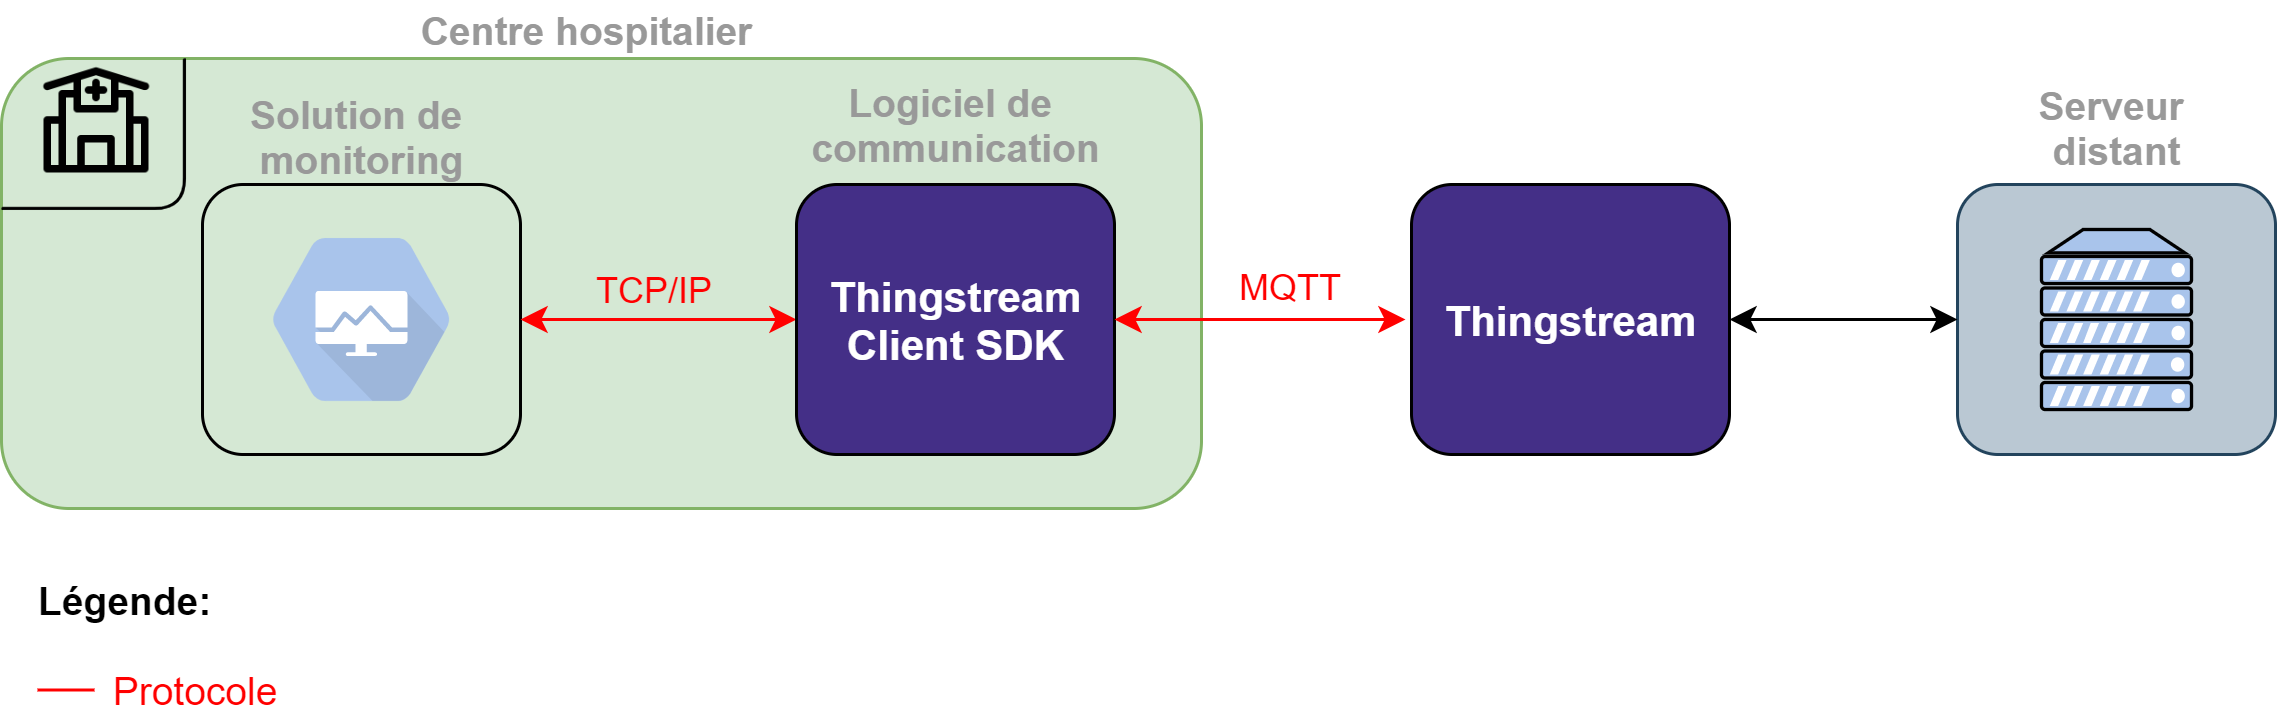
\includegraphics[width=\textwidth]{img/app/arch_start.png}
  \caption{Architecture après l'ajout du logiciel de communication}
  \label{fig:start_arch}
\end{figure}


~

\begin{figure}[ht!]
  \centering
  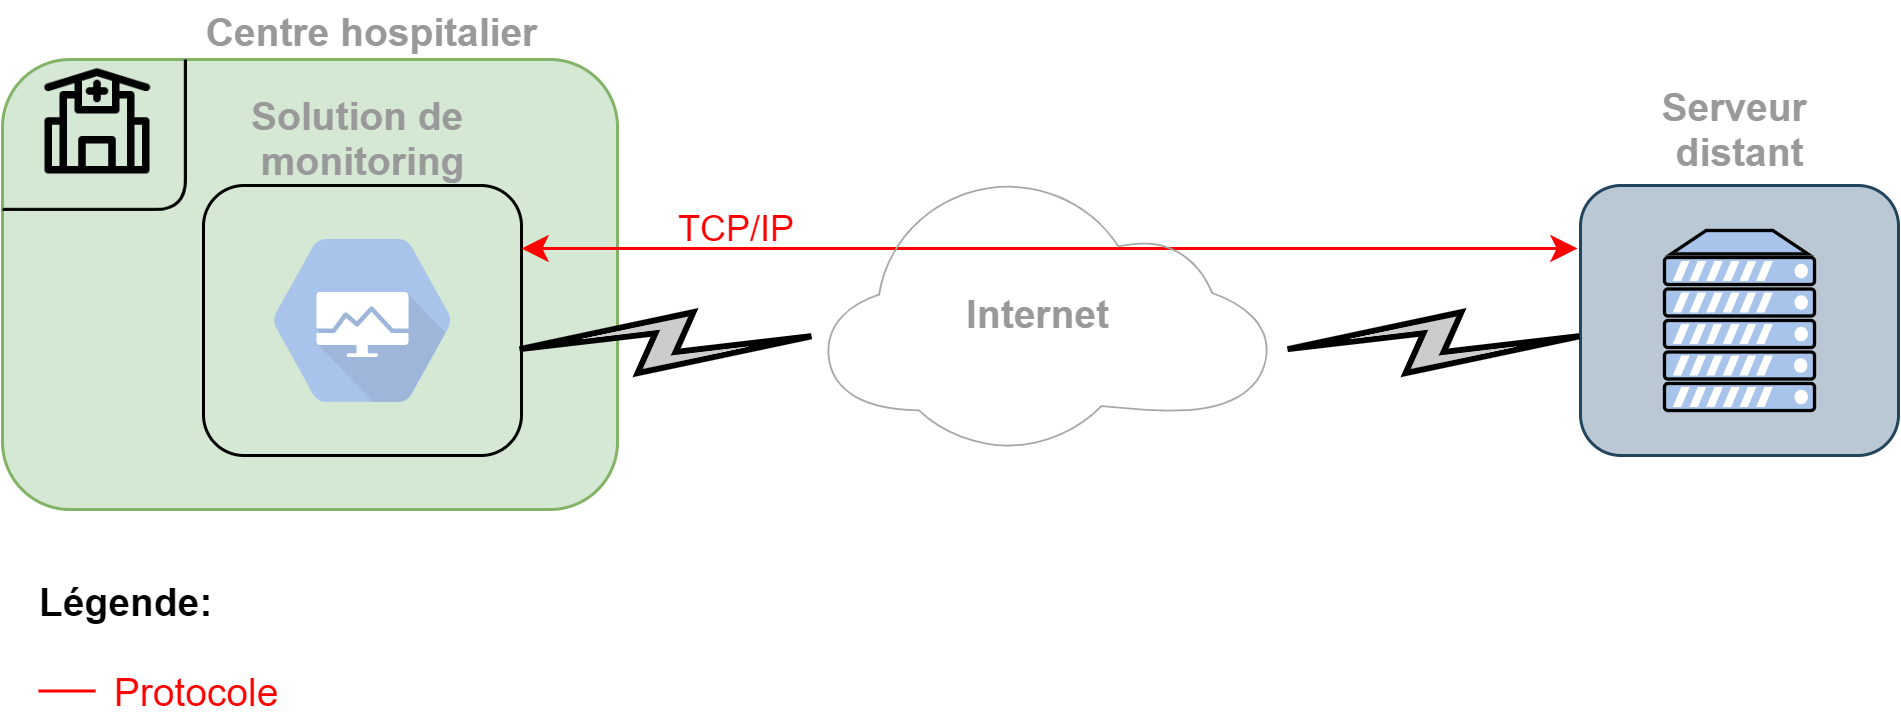
\includegraphics[width=0.8\textwidth ]{img/app/arch_no_thingstream.png}
  \caption{Architecture simplifiée de la solution de monitoring sans Thingstream}
  \label{fig:start_no_thing}
\end{figure}

\noindent
Ensuite il y a l'architecture de toute la solution de monitoring. Cette part comprend plusieurs fonctionnalités d'acquisition de données qui ne sont pas forcément liées entre elles. Par exemple, il y a l'acquisition de données concernant l'état du serveur ou la présence des tablettes. Cependant, certaines parties doivent pouvoir communiquer entre elles, comme le service de présence des tablettes et la fonction de mappage du réseau. En effet, le service de présence doit d'abord connaitre quels sont les dispositifs à monitorer et cela est accompli en regardant le résultat du mappage.


\noindent
Généralement, jusqu'à il y a quelques années, les applications avaient une architecture monolithique et des patrons de conception étaient utilisés pour séparer les diverses parties du logiciel. Au cours des dernières années, une nouvelle architecture a fait face, les microservices.  Cette conception se met en avant par le fait qu'elle brise les différents composants d'une application monolithique en plusieurs mini applications, aussi appelés les microservices. Ces services peuvent ensuite communiquer entre eux grâce à des protocoles distincts tels que HTTP, RPC\footnote{Remote procedure call} et RabbitMQ. La figure 1 reprend la différence entre les deux architectures.

~

\begin{figure}[ht!]
  \centering
  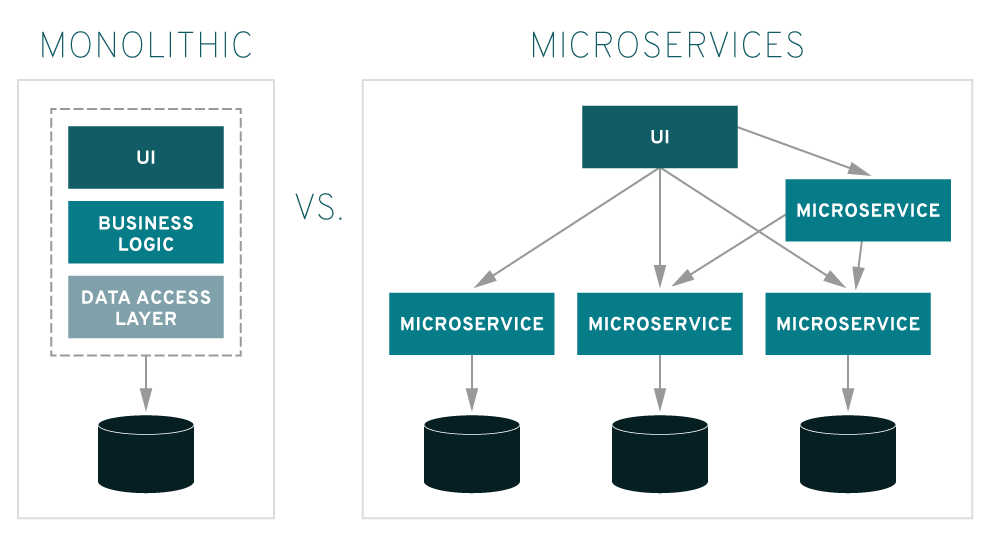
\includegraphics[width=0.8\textwidth]{img/app/monolithic-vs-microservices.png}
  \caption{Différence entre les architectures monolithique et microservices \cite{micro_diff}}
  \label{fig:monvsmicro}
\end{figure}

\noindent
Comparée à une architecture monolithique, les microservices possèdent les avantages suivants \cite{micro_diff} :

\begin{itemize}
  \item Mise sur le marché plus rapide
  \item Haute évolutivité
  \item Résilience
  \item Facilité de déploiement
  \item Accessibilité
  \item Ouverture
\end{itemize}

~

\noindent
Tous ces avantages sont particulièrement intéressants, particulièrement l'accessibilité, la haute évolutivité et la résilience. Ces trois grands avantages vont ensemble avec ce qui est requis pour ce projet. De ce fait, cette architecture est celle qui a été implémentée lors de ce mémoire. La section suivante couvrira chacun de ces microservices et comment ils interagissent entre eux.

~

\noindent
Cette section commence par la description de l'implémentation de chaque service. Ensuite, il sera question de la manière dont les services interagissent. Premièrement, les services en charge de la communication seront présentés puisque ce sont ceux qui ont été développés en premier. En effet, le choix d'utiliser Thingstream a été fait avant de considérer les solutions de monitoring possibles. Compte tenu des problèmes rencontrés avec la solution de communication l'année précédente, commencer par le développement de cette solution semblait être le choix plus judicieux. Cela signifie que la solution de monitoring s'adapte aux capacités de la solution de communication, et non l'inverse.


\subsection{Implémentation des fonctionnalités}

\subsubsection{Envoi des données}

\noindent
Comme expliqué dans la section \ref{sec:thingstream}, Thingstream propose un SDK qui permet de très aisément avoir accès la plateforme et de l'exploiter. Ce SDK gère toute la communication de bas niveau avec le modem, le SIM800L en l'occurrence. Son utilisation est très similaire à celle de toutes les autres bibliothèques logicielles de clients MQTT qui sont actuellement disponibles. Cette partie ne couvre donc que la façon dont un message est géré au niveau du protocole MQTT. À partir de cet instant, c'est le SDK de Thingstream qui s'en occupe et n'est donc pas discuté ici. Veuillez aussi noter que le choix de Thingstream a été effectué avant de démarrer le développement du logiciel de monitoring. Comme expliqué précédemment, la partie de communication a été très problématique lors du dernier projet. De ce fait, la décision fut d'adapter le logiciel à la solution de communication et non l'inverse étant donné la complexité de cette dernière.

~

\noindent
Dans le but de mieux comprendre le fonctionnement de la solution de communication, il faut d'abord découvrir les bases du protocole MQTT. Comme expliqué précédemment, ce protocole a été spécifiquement conçu pour être utilisé dans des réseaux non fiables. L'architecture du protocole MQTT est basée sur le patron de communication publish-subscribe. Des \textit{publishers}(éditeurs) publient des messages sur un topic et les \textit{subscribers}(abonnés) reçoivent tous les messages qui ont été publiés sur le topic auquel ils sont abonnés.  La figure \ref{fig:pub_sub} reprend un exemple de ce patron de communication. Deux \textit{publishers} publient un message sur deux topics différents. Le \textit{subscriber} A est seulement abonné au topic 1 et, par conséquent, ne reçoit que le message publié par le \textit{publisher} A. Cependant, le \textit{subscriber} B reçoit tous les messages puisqu'il est abonné aux deux topics. Les messages envoyés ne possèdent donc pas de destinataire en particulier. De plus, les \textit{publishers} ne savent pas a priori qui lira les messages qu'ils ont publiés.

~

\begin{figure}[ht!]
  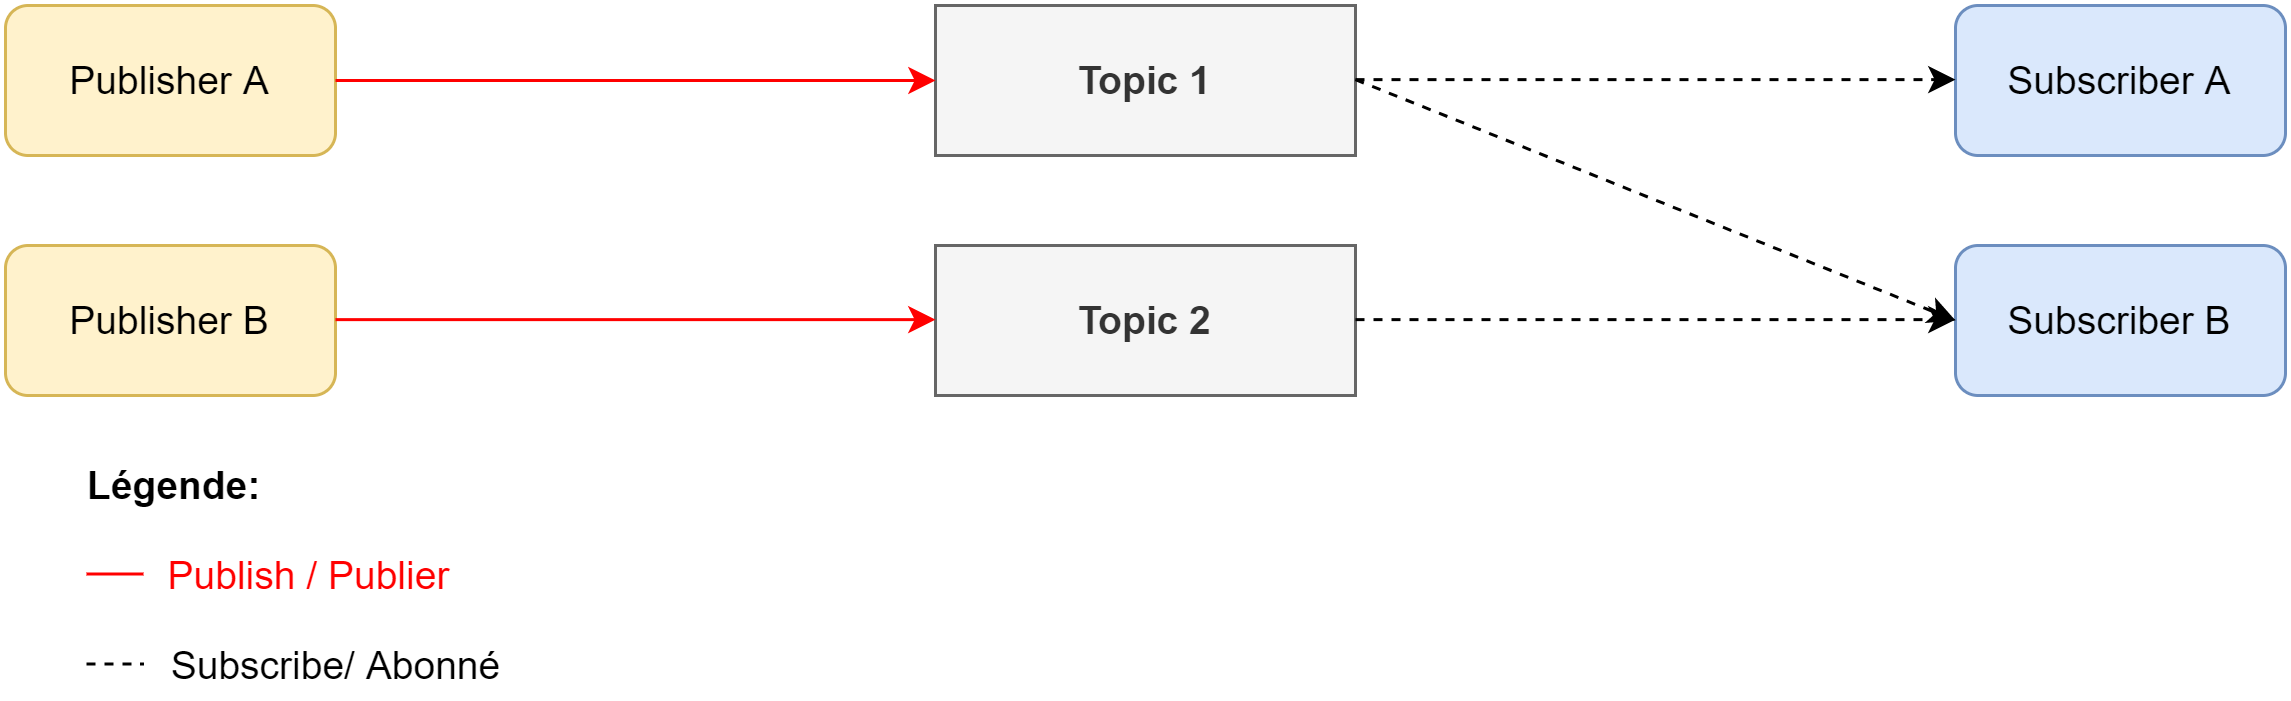
\includegraphics[width=\textwidth]{img/app/pub_sub.png}
  \caption{Patron de conception Publish-Subscribe}
  \label{fig:pub_sub}
\end{figure}


\noindent
Cette méthode permet de découpler les \textit{publishers} et les \textit{subscribers}. En effet, ils ne communiquent pas directement entre eux, mais font appel à une tierce partie, le \textit{broker}, pour échanger les messages. Au moment de la connexion, les \textit{subscribers} envoient au \textit{broker} la liste de topics auxquels ils veulent s'abonner. Lorsqu'un \textit{publisher} publie sur un topic, le \textit{broker} identifie tous les \textit{subscribers} souscrits à ce topic et leur transmet le message. La figure \ref{fig:pub_sub_seq} présente un diagramme de séquence de ce procès.

~

\begin{figure}[ht!]
  \centering
  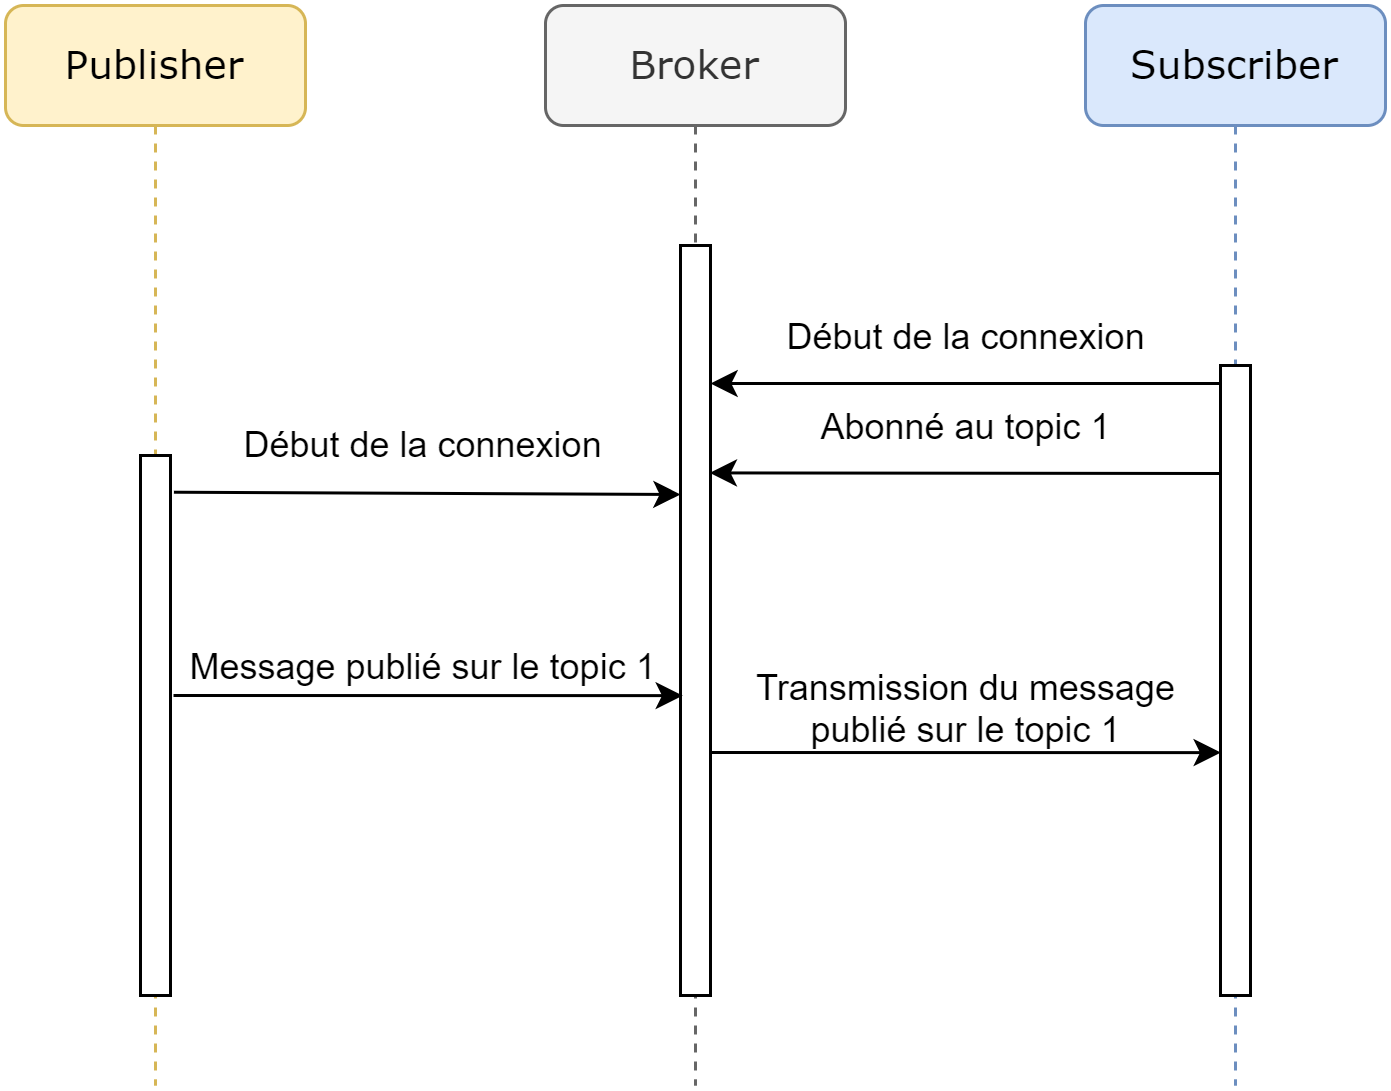
\includegraphics[width=0.7\textwidth]{img/app/process_pub_sub.png}
  \caption{Diagramme de séquence affichant un échange de données suivant le patron de conception Publish-Subscribe}
  \label{fig:pub_sub_seq}
\end{figure}


\noindent
Ceci constitue l'architecture de base du protocole MQTT. Cependant, les clients peuvent détenir les rôles de \textit{publisher} et de \textit{subscriber} à la fois, ils ne sont donc pas limités à une seule fonction. Un autre point important à comprendre à propos MQTT est la façon dont les topics fonctionnent. Un topic est représenté par une chaîne de caractères et il peut avoir plusieurs niveaux. Un caractère barre oblique (/) sépare chaque niveau. Par exemple, imaginons qu'un capteur de température se trouve dans le salon au rez-de-chaussée. La figure \ref{fig:ex_top} montre un exemple de topic qui pourrait être exploité par ce capteur pour transmettre ces données à travers le protocole MQTT. Cependant, supposons maintenant qu'un client veut s'abonner à tous les capteurs de température présents au rez-de-chaussée. Évidemment, ce client pourrait souscrire à chaque capteur individuellement. Pour éviter ce genre de situation, MQTT permet d'employer des wildcards pour qu'un client puisse s'abonner à plusieurs topics qui possèdent une structure similaire. Les figures \ref{fig:wildmq1} et \ref{fig:wildmq2} affichent la façon dont les wildcards peuvent être appliqués. Dans le logiciel de communication de ce mémoire, seulement le wildcard à niveau unique est utilisé.

~

\begin{figure}[ht!]
  \centering
  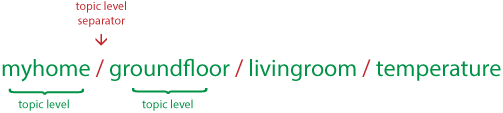
\includegraphics[width=0.5\textwidth]{img/app/example_topic.png}
  \caption{Exemple de topic MQTT \cite{mqtt_examples}}
  \label{fig:ex_top}
\end{figure}

~

\begin{figure}[ht!]
  \centering
  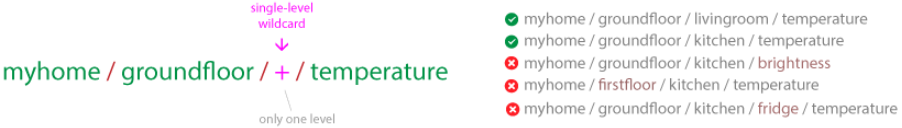
\includegraphics[width=0.85\textwidth]{img/app/mqtt_wild1.png}
  \caption{Exemple d'utilisation du wildcard à niveau unique pour matcher plusieurs topics \cite{mqtt_examples}}
  \label{fig:wildmq1}
\end{figure}

~

\begin{figure}[ht!]
  \centering
  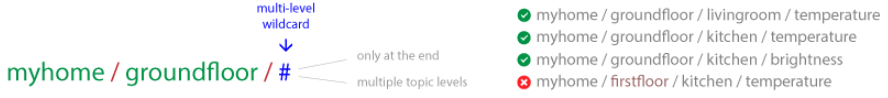
\includegraphics[width=0.85\textwidth]{img/app/mqtt_wild2.png}
  \caption{Exemple d'utilisation du wildcard de plusieurs niveaux pour matcher plusieurs topics \cite{mqtt_examples}}
  \label{fig:wildmq2}
\end{figure}


\noindent
Le protocole MQTT possède encore d'autres fonctionnalités comme la qualité de service. Toutefois, ces fonctionnalités supplémentaires n'ont pas été exploitées lors de ce mémoire et ne sont donc pas spécifiées ici. Veuillez aussi noter que le client décrit dans cette section emploie MQTT-SN, et non pas la version standard de MQTT. En effet, ce client est ce que Thingstream appelle un SN-Thing. Cela dit, le fonctionnement des deux protocoles est très similaire. Contrairement à MQTT, MQTT-SN utilise des alias pour remplacer le nom complet des topics et permet aux clients de se déconnecter temporairement dans le but d'économiser de l'énergie. Les messages qui devraient être envoyés au client sont alors sauvegardés dans le broker jusqu'à la reconnexion du client. Les sources proposent des informations plus détaillées sur MQTT et MQTT-SN. La dernière spécification complète de MQTT peut être trouvée dans \cite{banks2019mqtt}.

~

\noindent
Le client de communication développé exploite trois topics afin de transmettre des informations. Tous les messages sont encodés dans le format de données JSON\footnote{JavaScript Object Notation}, indépendamment du topic. Ce format est facilement lisible par un humain et est supporté par la majorité des langages de programmation. En outre, son utilisation est très répandue sur le web. Cependant, selon le topic, la structure du JSON est différente. Ci-dessous est présentée la liste des trois topics et le format de données utilisé dans chacun d'eux\footnote{\#identity\# est un ID unique attribué par Thingstream à chaque client} :

~

\begin{itemize}
  \item \textbf{/device/\#identity\#/startup} : Le client utilise ce topic lorsque l'application exploitant le client de communication doit s'authentifier auprès du serveur. Les messages publiés sur ce topic ont la forme suivante :
\end{itemize}

\begin{lstlisting}[language=json]
{
  "id" : #id#,
  "location" : #localisation_dispostif#
}
\end{lstlisting}

~

\begin{itemize}
  \item \textbf{/device/\#identity\#/post} : Ce topic est utilisé afin de transmettre les données envoyées par l'application au serveur. Un en-tête doit être ajouté à tous les messages publiés sur ce topic afin d'identifier le type des données publiés. La structure des messages est la suivante :
\end{itemize}

\begin{lstlisting}[language=json]
{
  "type" : #type_contenu#,
  "content" : [ #donnees# ]
}
\end{lstlisting}

~

\begin{itemize}
  \item \textbf{/device/all/sms} : : Ce topic est utilisé pour envoyer des SMS au techniciens. Contrairement aux deux topics précédents, le serveur n'est pas souscrit à ce topic. En effet, c'est un Data Flow de Thingstream qui y est abonné. Tous les messages publiés sur ce topic sont convertis en un SMS qui est envoyé à un récipient. De ce fait, les champs du JSON sont différents de ceux du topic post. Le Data Flow est affiché dans la figure \ref{fig:flow} et la structure d'un message publié sur ce topic est la suivante :
\end{itemize}

\begin{lstlisting}[language=json]
{
  "message" : #contenu_sms#,
  "to" : #numero_gsm_recipient#
}
\end{lstlisting}

~

\begin{figure}[ht!]
  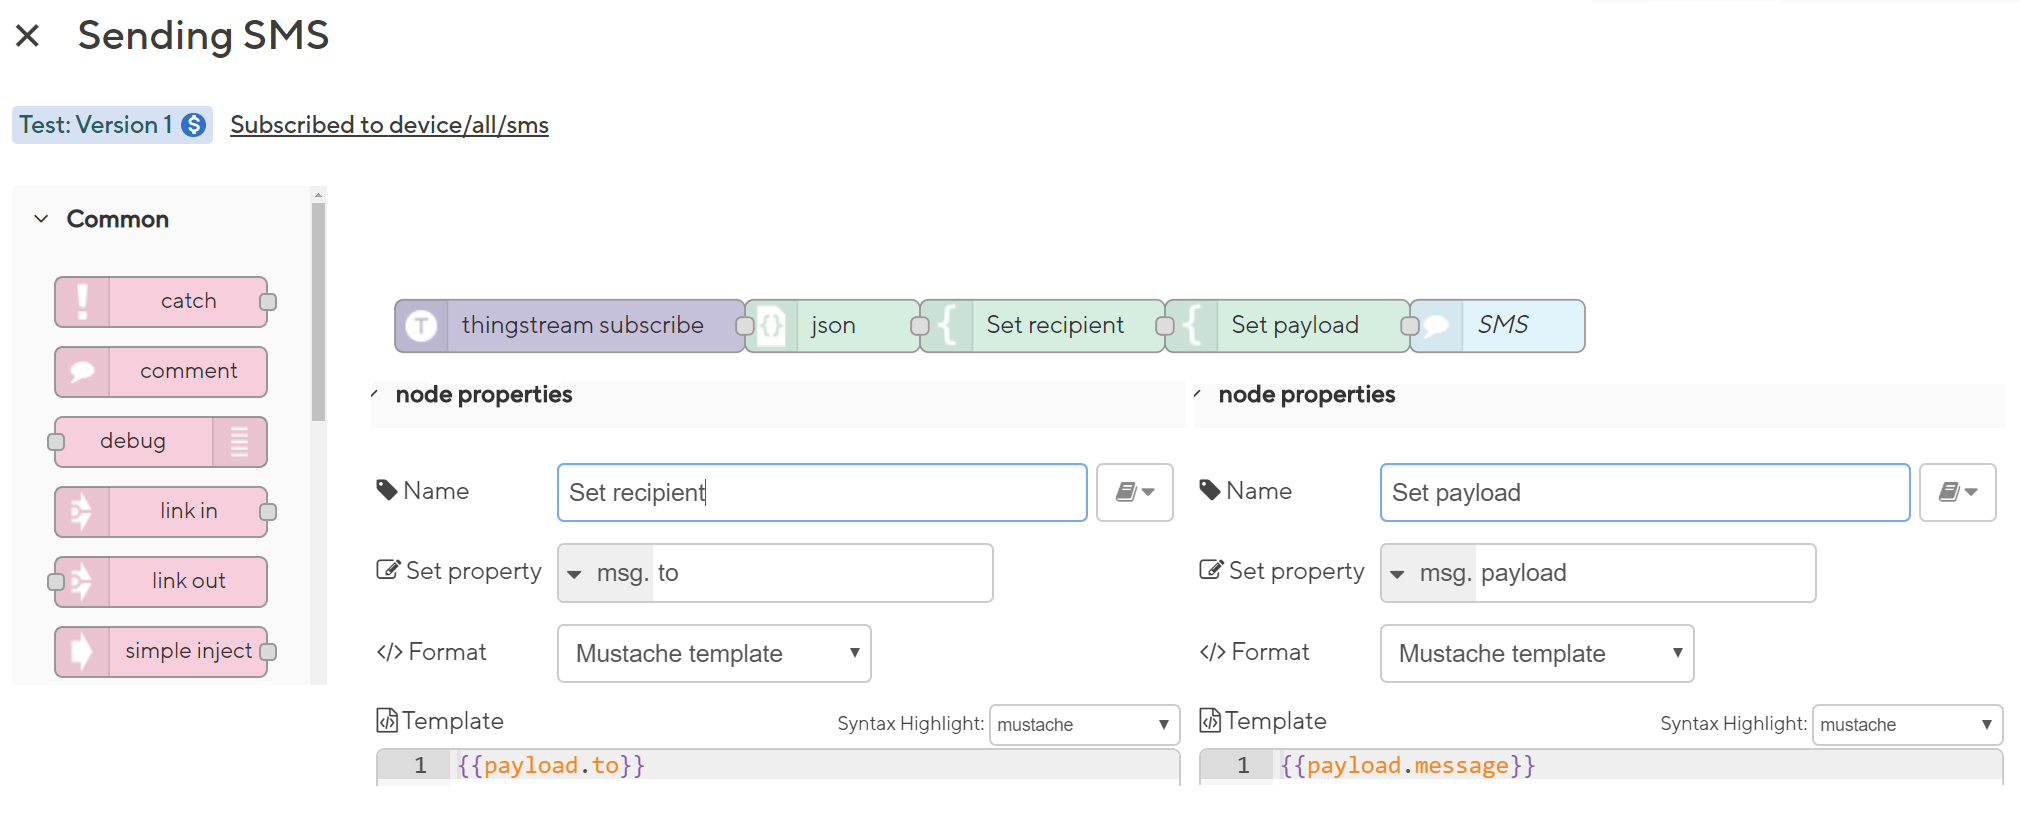
\includegraphics[width=\textwidth]{img/app/data_flow.png}
  \caption{Exemple de Data Flow de Thingstream permettant d'envoyer un SMS}
  \label{fig:flow}
\end{figure}


\noindent
En plus des trois topics sur lesquels le client publie des messages, le client s'abonne à un quatrième topic afin que le serveur puisse lui adresser des messages. Ce topic est \textbf{device/\#identity\#/recv} et sera expliqué plus en détail dans la section \ref{sec:server}. Toutes les informations reçues par le client de communication sur ce topic sont transmises au logiciel de monitoring.

~

\noindent
Comme défini dans l'architecture du programme, l'application de communication est complètement isolée et accepte les connexions sur un socket de serveur TCP/IP. Par conséquent, la solution de monitoring ne possède aucune information sur le fonctionnement du logiciel de communication décrit ci-dessus. Il ne fait qu'envoyer les données sur le socket et le laisse le client de communication se charger du reste. Cependant, elles possèdent deux destinataires possibles, le serveur distant ou le récipient des SMS. Dans le but de créer une distinction entre ces deux types de messages, ils sont encapsulés par un autre JSON qui a la forme suivante :

\begin{lstlisting}[language=json]
{
  "type" : "server" ou "sms",
  "payload" : #numero_gsm_recipient#
}
\end{lstlisting}

~

\noindent
Cette capsule est lue par le client de communication qui décide ensuite sur quel topic il faut publier le message, mais seulement le contenu du champ \textit{payload} est publié.

~

\noindent
Un dernier aspect important de ce client de communication est qu'il permet à une seule application de se connecter à la fois au serveur distant. Créer un client capable de gérer des connexions augmenterait considérablement sa complexité sans apporter aucun avantage au projet. Mais, puisque le client n'accepte qu'une seule connexion, il doit s'assurer que c'est bien celle du logiciel de monitoring qui est approuvé. C'est pourquoi un protocole a été mis en place qui permet d'authentifier l'application auprès du serveur. Le diagramme de séquence de la figure \ref{fig:seq111} présente le déroulement du protocole.




~

\noindent
Du côté de l'application de monitoring, un service unique reçoit toutes les données et se charge de les transmettre au client de communication. Avant la transmission, il formate les données en fonction du destinataire et du type de données. Le fonctionnement exact de ce service sera détaillé au cours des section suivantes et il sera identifié par le nom \textit{sender service}. La figure \ref{fig:sender_arch} présente l'architecture complète après l'introduction du \textit{sender service} et le service de communication.

\begin{figure}[ht!]
  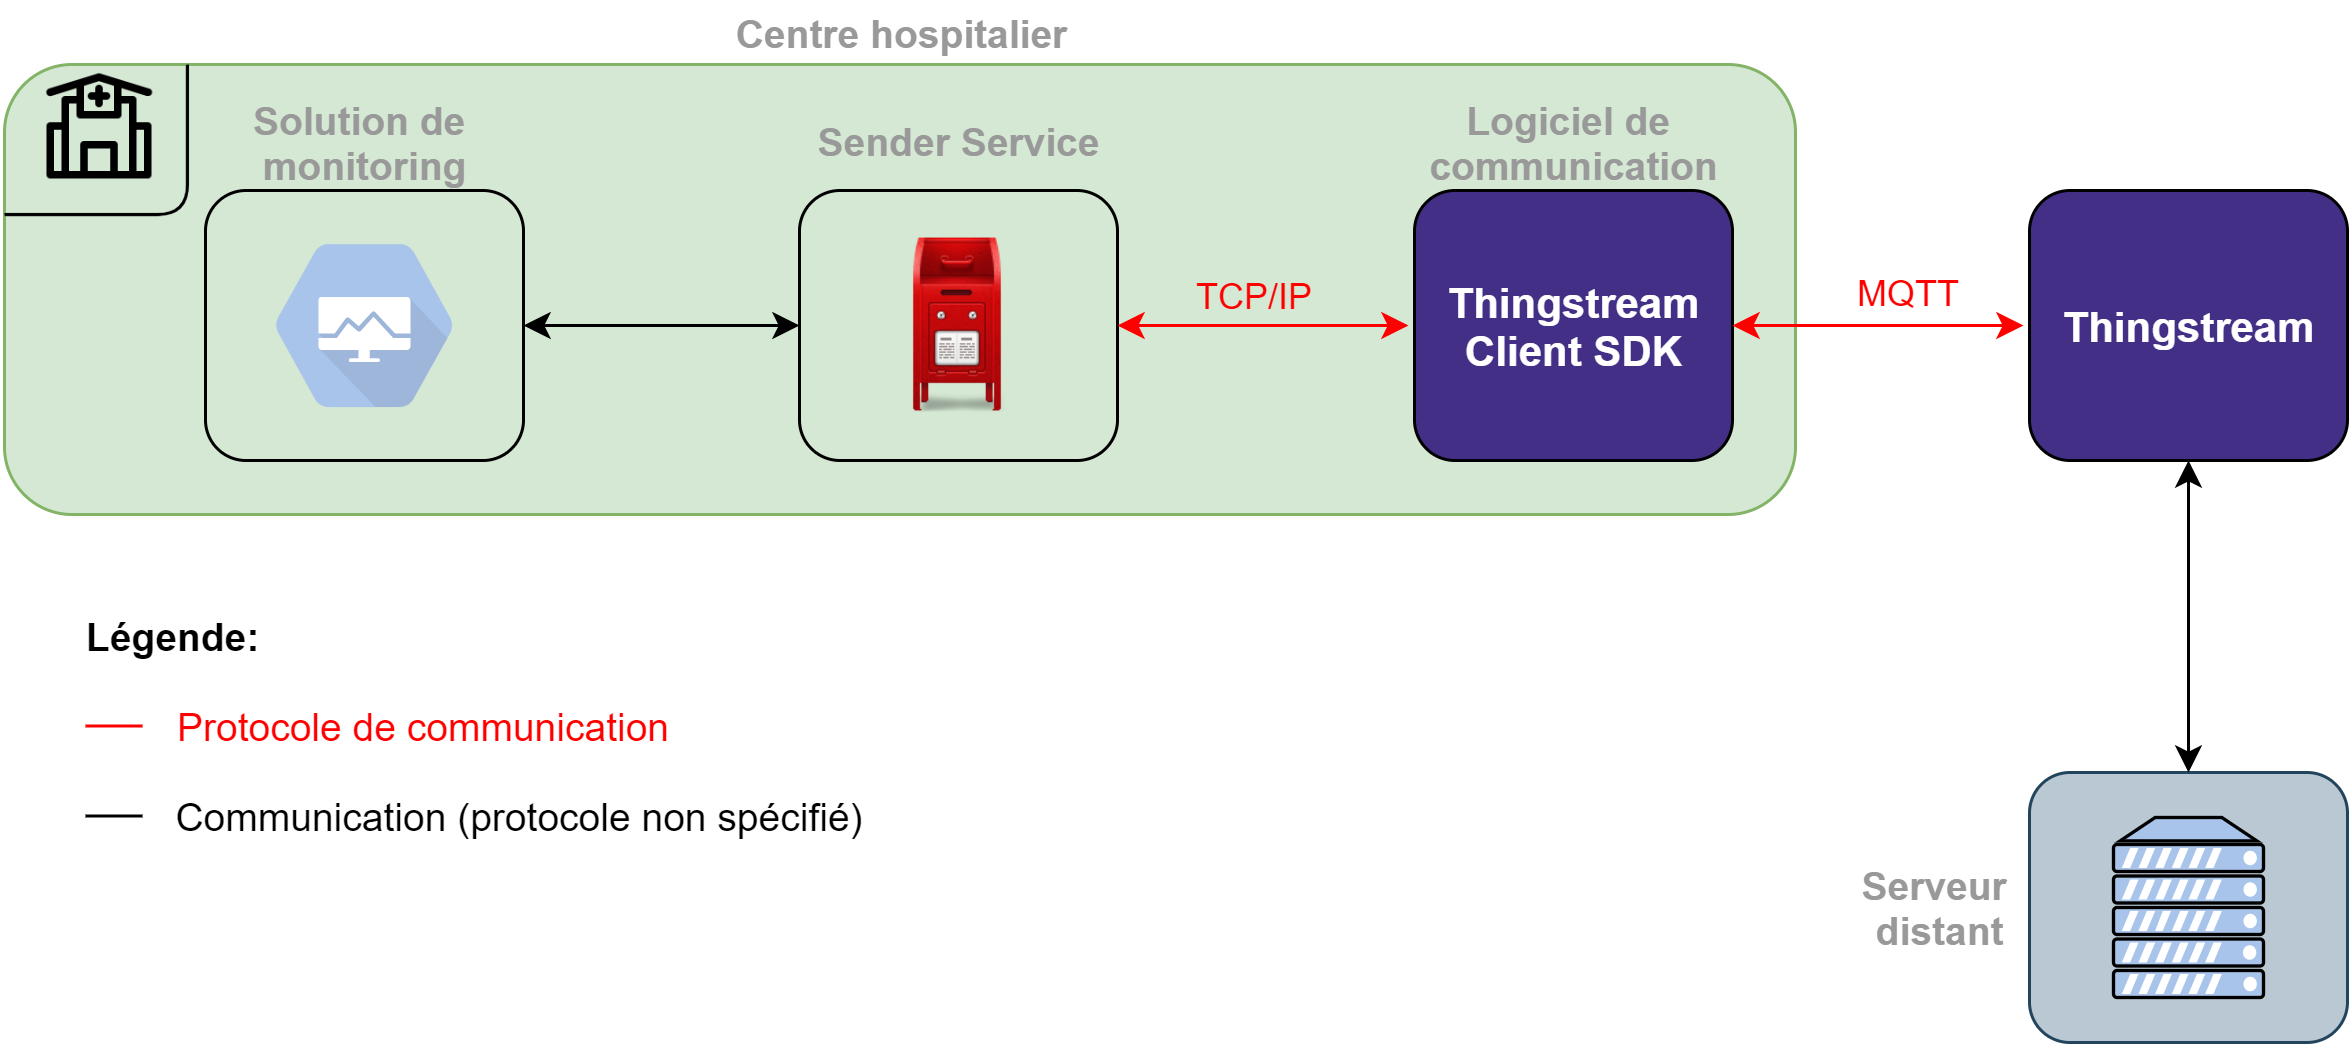
\includegraphics[width=\textwidth]{img/app/sender_arch.png}
  \caption{Architecture après l'ajout du \textit{sender service}}
  \label{fig:sender_arch}
\end{figure}


\begin{figure}[ht!]
  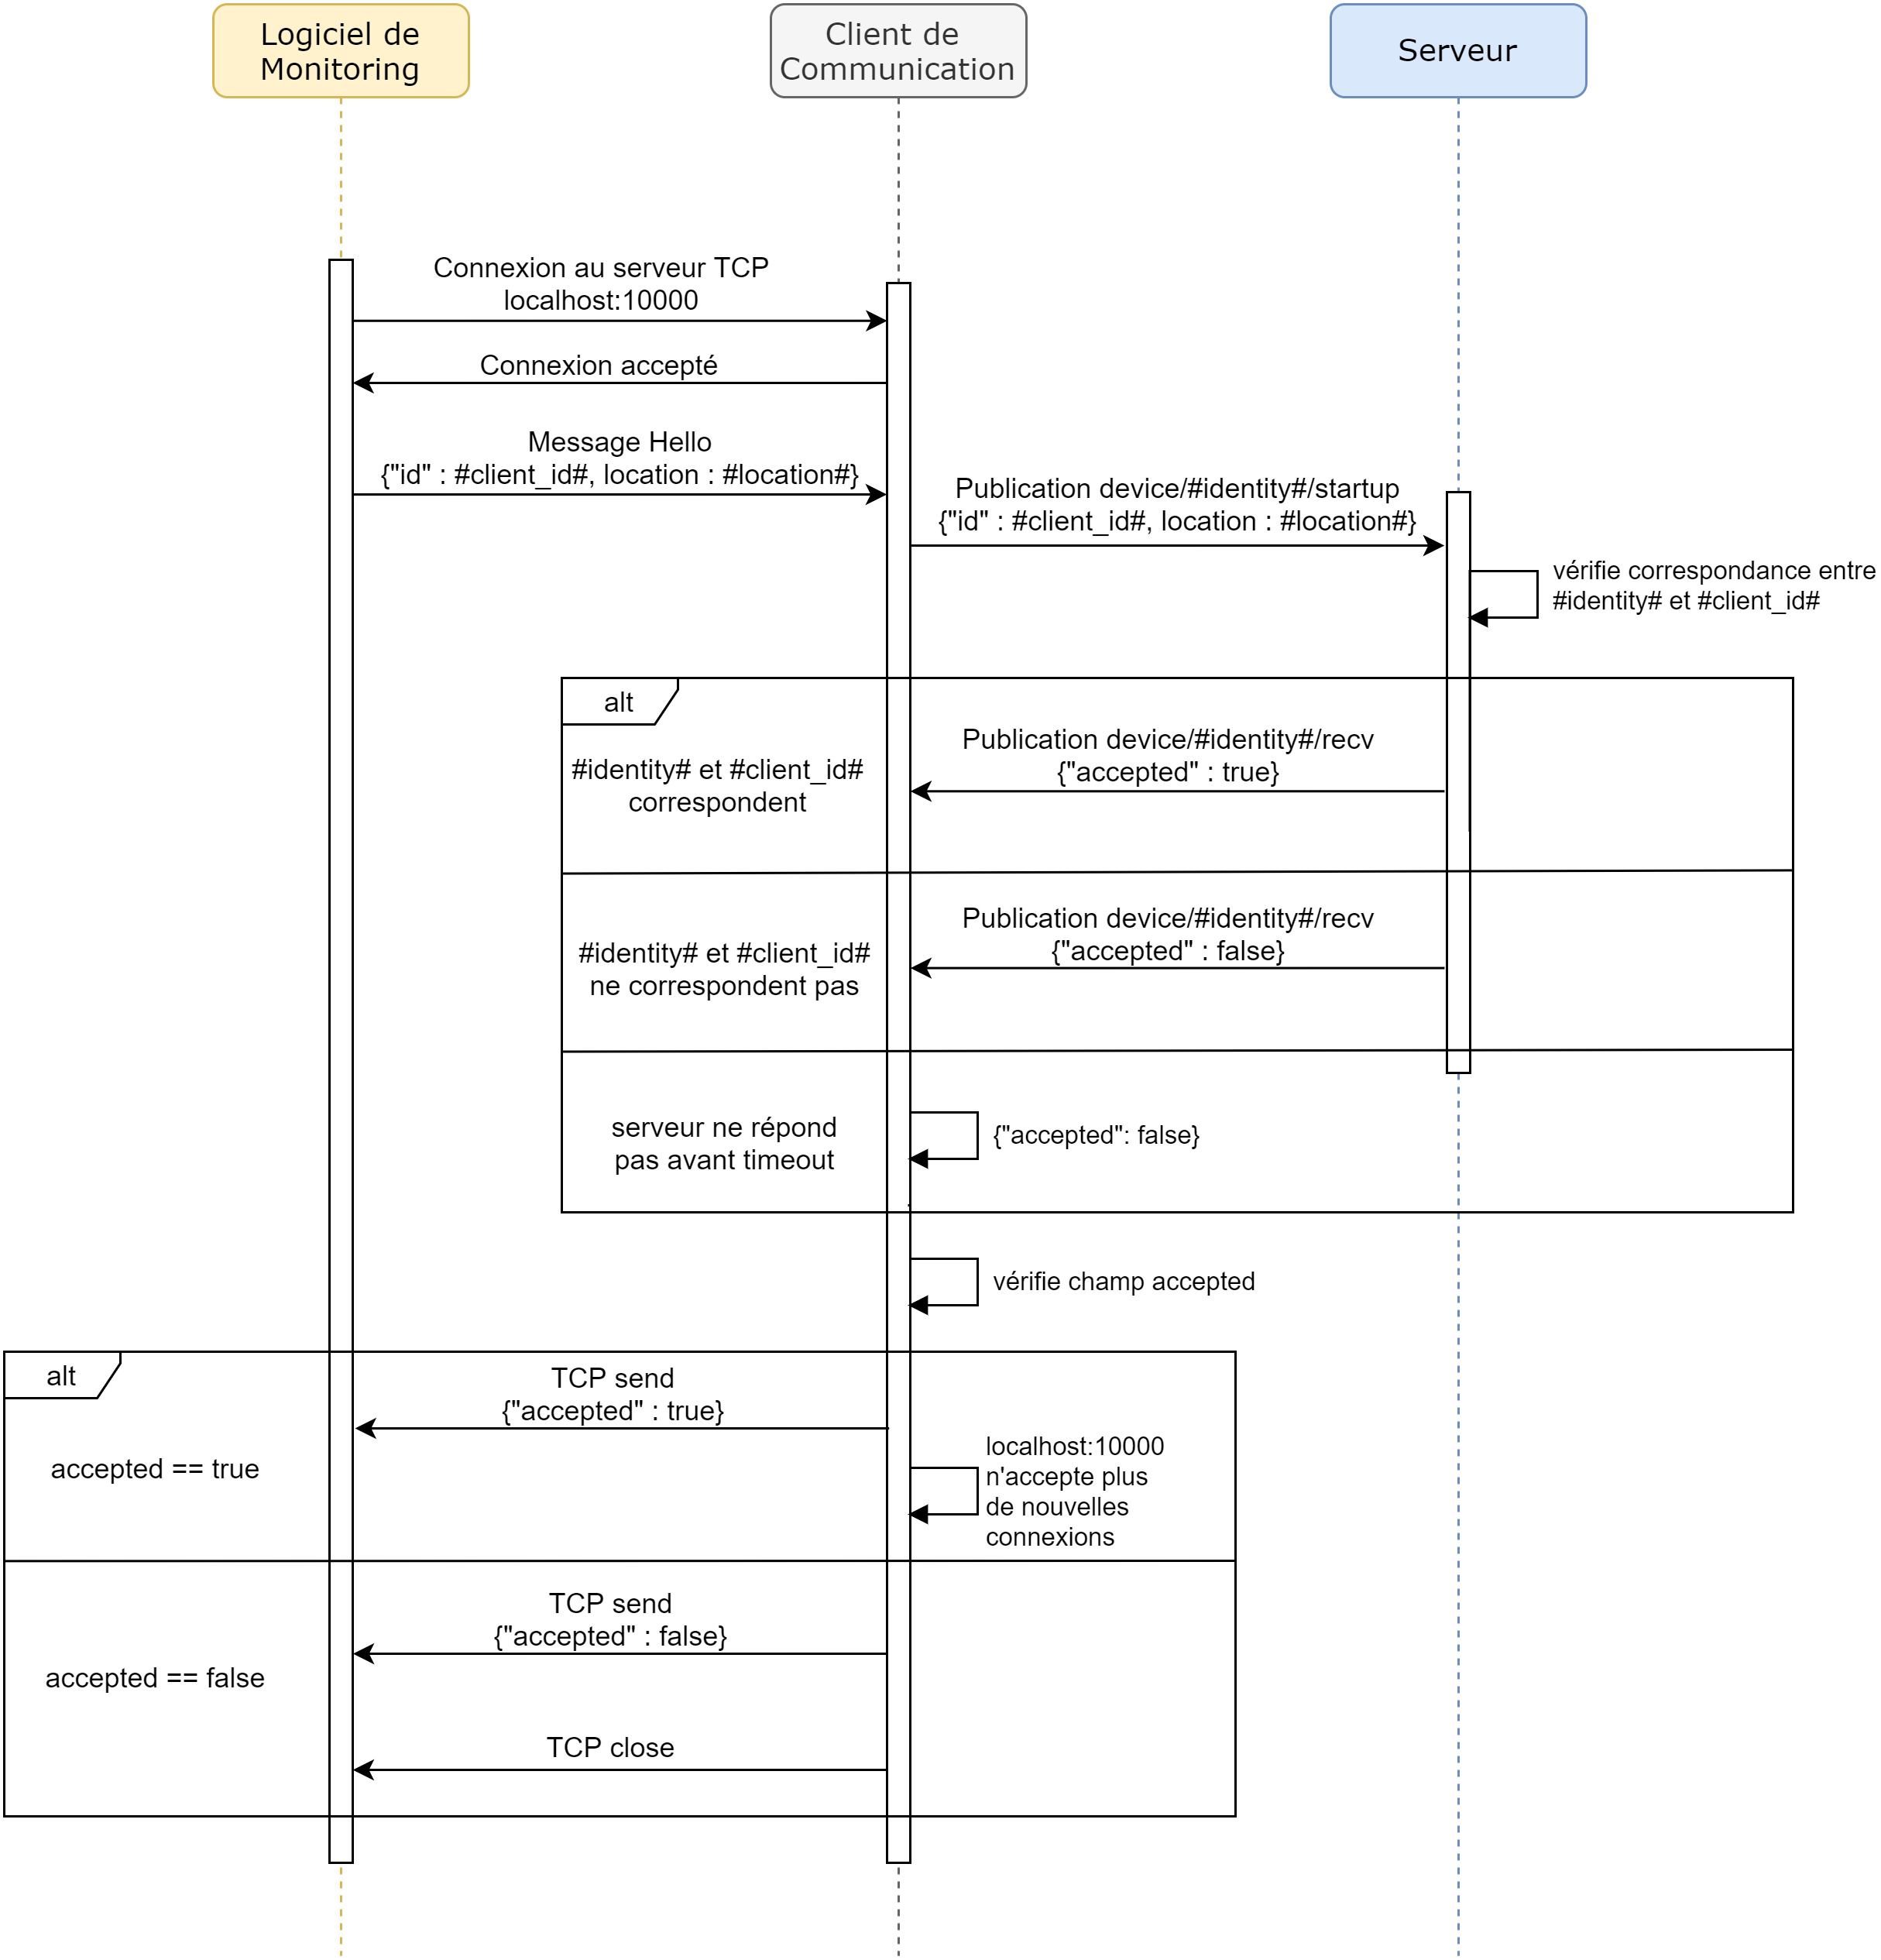
\includegraphics[width=\textwidth]{img/app/con_protocol.png}
  \caption{Diagramme de séquence à propos le processus de connexion au serveur distant}
  \label{fig:seq111}
\end{figure}

\newpage
\newpage


\subsubsection{Monitoring du serveur}

\noindent
Dans l'intention de surveiller l'état du serveur, le protocole SNMP \footnote{Simple Network Management Protocol} a été utilisé lors des projets antérieurs. Ce protocole a été conçu spécifiquement pour surveiller, diagnostiquer et administrer des dispositifs. Presque tous les types d'appareils connectés à un réseau IP sont pris en charge, y compris les serveurs, les imprimantes et les routeurs. Puisque le cahier des charges ne stipule qu'un nombre réduit de métriques du serveur à surveiller, le protocole SNMP s'est montré comme une solution simple à implémenter. Bien entendu, étant une solution existant depuis un bon nombre d'années, la majorité des langages de programmation propose des bibliothèques logicielles pour exploiter SNMP.

~

\noindent
Lors de ce mémoire, une première implémentation utilisant SNMP pour récupérer les valeurs du serveur a été réalisée. Ce logiciel était capable de retrouver toutes les valeurs précisées dans le cahier des charges sans présenter aucun problème. Cependant, cette solution manquait d'évolutivité. En effet, une quantité de code considérable était déjà requise pour récupérer, traiter et sauvegarder l'\textit{uptime} du serveur ainsi que l'état des processus. En outre, les parties prenantes du projet avaient exprimé le souhait de disposer d'une application hautement configurable au niveau de la définition des alertes. Ce dernier aspect augmentait encore plus la complexité du système.

~

\noindent
Trouver une meilleure solution est alors devenu primordial. Pour ce faire, les différents logiciels de monitoring disponibles sur le marché ont été étudiés. Quelques critères ont été établis en vue d'identifier celui qui est le plus adapté à ce projet. Premièrement, la solution devrait être entièrement gratuite. Plusieurs solutions payantes existent, mais leur coût est très important. Deuxièmement, le logiciel devrait être facile à utiliser et présenter une bonne et ample documentation. Ensuite, il devrait être hautement configurable, permettant de l'ajuster aux besoins de CERHIS. Finalement, le logiciel devrait être compatible avec le plus grand nombre possible d'appareils de CERHIS.

~

\noindent
Après avoir posé ces critères, trois solutions sont ressorties :

~

\begin{itemize}
  \item \textbf{Prometheus} est un logiciel open source de monitoring et \textit{alerting toolkit} qui est actuellement maintenu par la Cloud Native Computing Foundation\footnote{CNCF}. Prometheus est basé sur le modèle \textit{pull}, mais offre aussi la possibilité de l'utiliser avec le modèle \textit{push}. Quelques fonctionnalités très intéressantes proposées par ce logiciel sont la base de données orientée séries temporelles, un modèle de données multidimensionnelles et la compatibilité avec Grafana. Prometheus est une solution très récente, créée seulement en 2012 et passée sous la responsabilité de la CNCF en 2016. De ce fait, son paradigme est différent des applications de monitoring traditionnelles. Prometheus se concentre sur les services \cite{prometheus_paradigm} contrairement aux applications classiques qui ont principalement la machine en tête.

  ~

  \item \textbf{Zabbix} est aussi un logiciel open source existant depuis 2001 et conçu pour le monitoring des divers dispositifs IT. Son architecture est basée sur le modèle \textit{push}. Zabbix exploite un large spectre de protocoles afin de surveiller une infrastructure IT. En outre, des agents sont également proposés pour une grande variété de plateformes, notamment des agents pour les systèmes d'exploitation Linux et Android. Par rapport à Prometheus, cette solution est un peu plus traditionnelle, même si elle reçoit des mises à jour assez régulièrement. Une interface graphique permettant de configurer le monitoring et de visualiser les données est incluse.

  ~

  \item \textbf{PandoraFMS Community}, tout comme les deux autres propositions, est aussi un logiciel open source. Cependant, cette solution possède également une version payante avec des fonctionnalités supplémentaires. Étant une solution disponible sur le marché depuis 2004, cette solution est très similaire à Zabbix. Ces deux plateformes possèdent quelques fonctionnalités exclusives, mais elles ne sont pas intéressantes dans le cadre de ce projet. D'un point de vue du logiciel, Pandora est la solution qui a besoin de plus de ressources.
\end{itemize}


~

\noindent
Pour finir, le choix s'est porté sur Prometheus. PandoraFMS a été éliminé assez rapidement, car cette solution est plus gourmande en ressources. De plus, l'image PandoraFMS pour le Raspberry Pi semble être payante. (La documentation n'est pas super claire sur cet aspect) L'agent Android proposé par Zabbix était le plus grand atout de cette solution. Cependant, certains de ces agents sont payants et ils sont tous proposés par de tierces parties. En outre, ils ne sont pas mis à jour très souvent et leur documentation est très limitée.

~

\noindent
Prometheus ressort donc comme étant le choix le plus sûr. Tous les clients \textit{exporters} disponibles pour cette solution sont open source, mais créer des clients supplémentaires est également très facile. En effet, une bibliothèque logicielle est disponible en plusieurs langages de programmation, ce qui rend l'implémentation très facile. De plus, Prometheus peut également être utilisé comme une simple base de données orientée séries temporelles. Cela permet donc de sauvegarder des valeurs comme la tension de la batterie de CERHIS sans devoir recourir à d'autres bases de données.

~

\noindent
L'architecture de Prometheus est présentée sur la figure \ref{fig:prom_arch}. Comme expliqué précédemment, Prometheus \textit{pull} des métriques au niveau des différents services. Ces services peuvent exporter des valeurs liées à l'état d'une machine, d'une application, d'une base de données ou de n'importe quel autre composant pouvant être surveillé par des métriques. Afin de \textit{pull} les données, Prometheus utilise le protocole HTTP.

\begin{figure}[ht!]
  \centering
  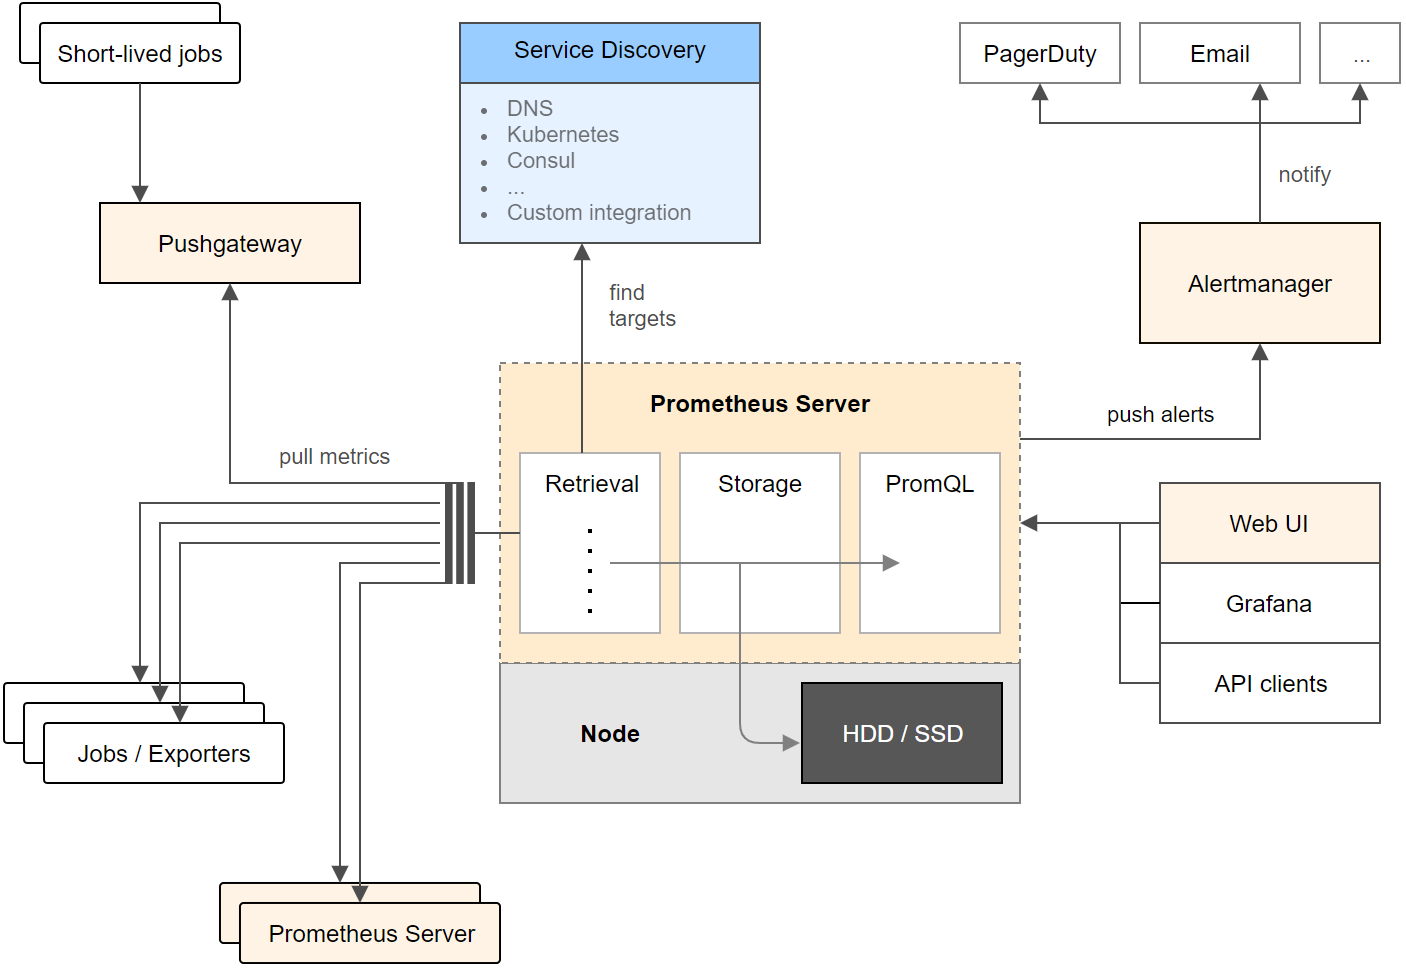
\includegraphics[width=0.9\textwidth]{img/app/prom_arch.png}
  \caption{Architecture de Prometheus}
  \label{fig:prom_arch}
\end{figure}

~

\noindent
Lorsque la méthode \textit{pull} ne peut pas être utilisée pour communiquer avec certains services, Prometheus propose d'utiliser le Pushgateway. Les services peuvent alors \textit{push} les données sur le Pushgateway et Prometheus effectuera le \textit{pull} au niveau de ce dernier. Cette solution est particulièrement intéressante pour surveiller les tablettes. En effet, le système d'exploitation Android peut mettre en pause des services afin d'économiser de la batterie (mode Doze, voir section \ref{sec:projet_precedent}). Cela rend la méthode \textit{pull} inutilisable puisqu'il est impossible de prédire quand le service sera disponible. Le dispositif Android doit donc utiliser la méthode \textit{push} pour envoyer les données dans les fenêtres de temps autorisés par le système d'exploitation. Malheureusement, actuellement aucun \textit{exporter} de données n'est disponible pour Android, mais il pourrait être développé.

~

\noindent
Prometheus peut aussi \textit{pull} des données auprès d'une deuxième instance de Prometheus possiblement tournant dans un autre appareil. \footnote{support for hierarchical and horizontal federation} Par exemple, ceci est intéressant si des multiples instances sont déployées dans plusieurs localisations. En effet, cette fonctionnalité permet d'utiliser une instance Prometheus maître qui centralise toutes les données des instances esclaves. Un exemple de cette architecture de fédération est donné dans la figure \ref{fig:prom_fed}. Cependant, une connexion à Internet est requise si les deux instances ne se trouvent pas dans le même réseau local.


\begin{figure}[ht!]
  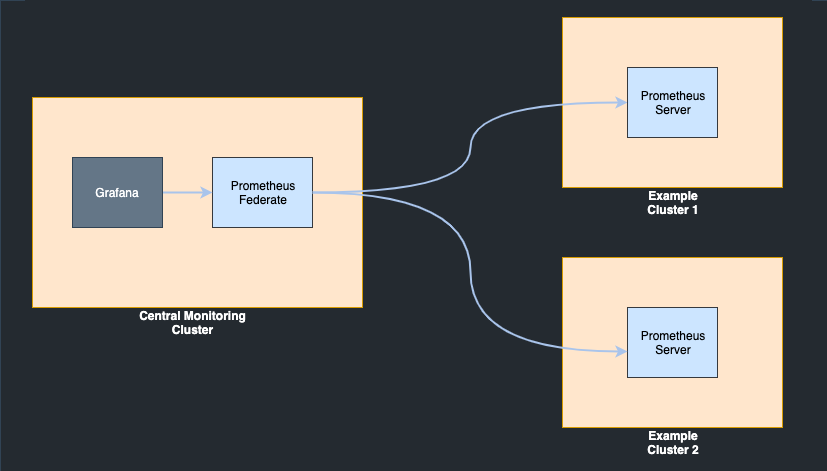
\includegraphics[width=\textwidth]{img/app/prometheus_federate.png}
  \caption{Architecture de fédération de Prometheus \cite{prometheus_federation}}
  \label{fig:prom_fed}
\end{figure}

~

\noindent
Finalement, un des outils plus importants de Prometheus est l'Alertmanager. En effet, grâce à des fichiers de configuration YAML, il est possible de définir des conditions d'alerte et le comportement à adopter lorsqu'elles se produisent. Le Listing \ref{lst:alert} affiche un exemple de la manière dont une telle alerte peut être configurée. En l'occurrence, cette configuration vérifie si le serveur a redémarré au cours des dernières 10 minutes et génère une alerte si c'est le cas. L'Alertmanager, comme son nom l'indique, collecte et traite toutes les alertes générées. De plus, ce dernier peut aussi transmettre des messages d'alertes par email, par messages Slack ou par des webhooks. Cette dernière fonctionnalité est très intéressante, car elle permet donc de créer un service local qui peut être contacté à travers un webhook.

\begin{listing}

  \begin{minted}[
  frame=lines,
  framesep=2mm,
  baselinestretch=1.2,
  bgcolor=background,
  fontsize=\footnotesize,
  linenos]{yaml}
  groups:
  - name: Default Server Monitoring
    rules:
    - alert: ServerRestart
      expr: node_boot_time_seconds != node_boot_time_seconds offset 10m
      for: 2m
      labels:
        severity: critical
      annotations:
        summary: "Instance {{ $labels.instance }} was down very recently"
        description: "{{ $labels.instance }} of job {{ $labels.job }} restarted
        at least once in the past 10 minutes"
        message: 'Serveur {{ $labels.instance }} a redemarre au moins une fois
        lors des dernieres 10 minutes '
  \end{minted}

\caption{Configuration de l'alerte relative au redémarrage du serveur}
\label{lst:alert}

\end{listing}

~

\noindent
C'est cette approche qui a été implémentée dans ce mémoire puisque le Raspberry Pi n'a pas accès à Internet. De ce fait, un service local, l'\textit{alert filter and collector service}, reçoit tous les messages d'alerte envoyés par l'Alertmanager et puis il se charge de les transmettre au service de communication. Le REST API webhook de ce service a été implémenté en utilisant le web framework Flask. La figure \ref{fig:archprometheus} présente l'architecture complète de cette solution. Vous pouvez aussi remarquer que Grafana a été utilisé en tant qu'outil pour la visualisation de données. En effet, cet outil supporte la base de données de Prometheus ce qui rend le processus de configuration extrêmement simple.

\begin{figure}
  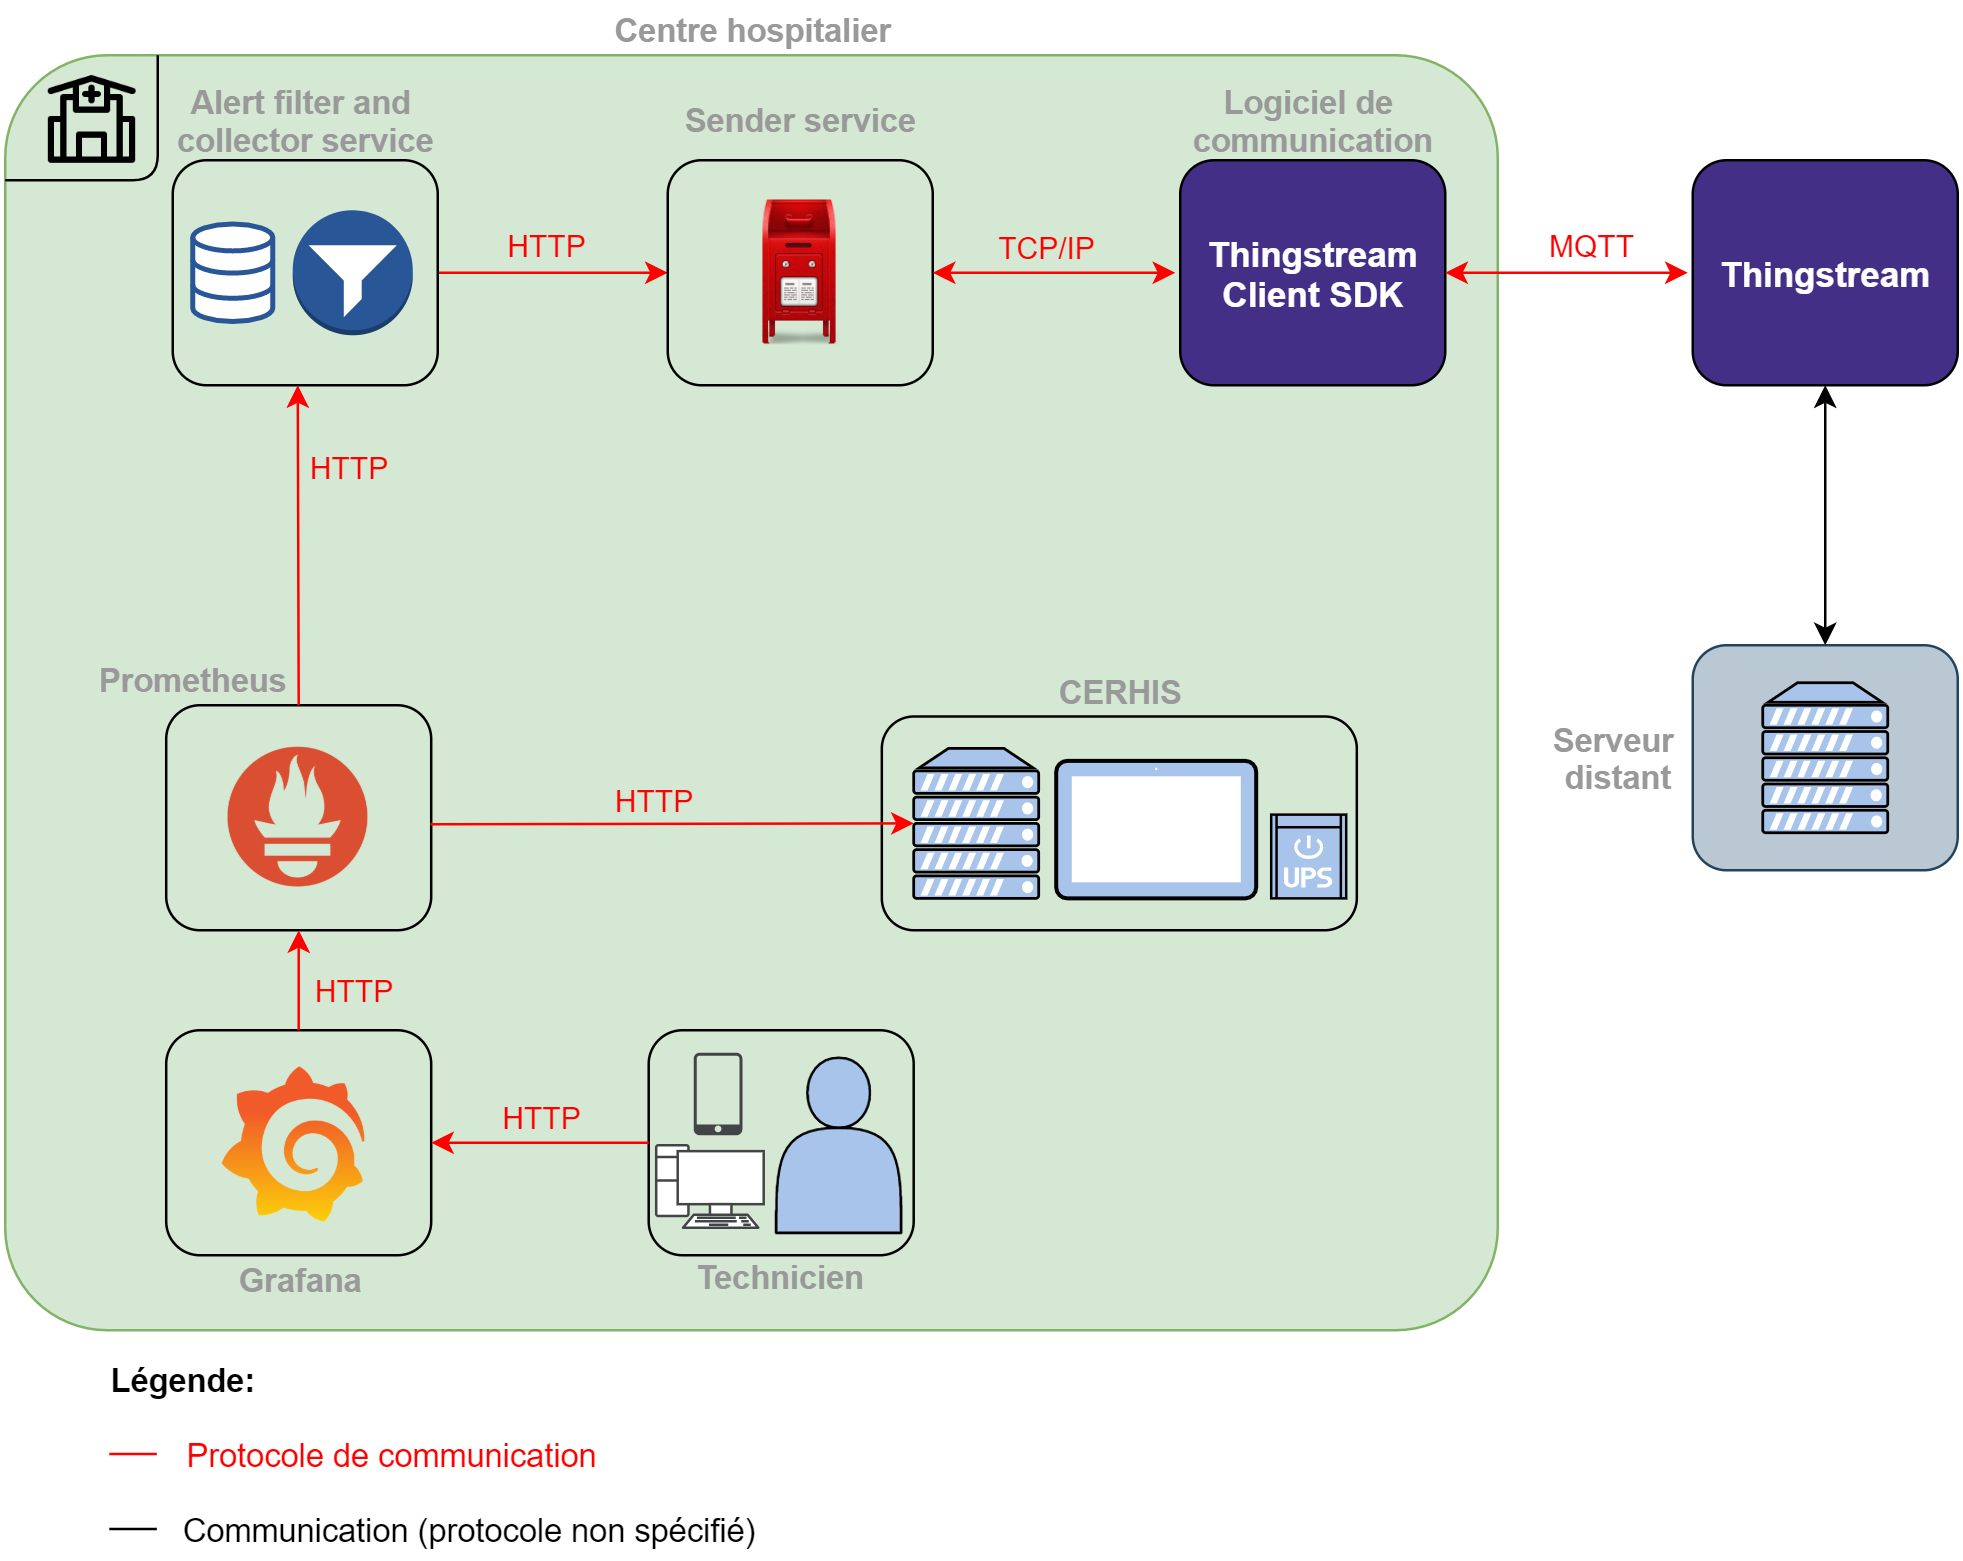
\includegraphics[width=\textwidth]{img/app/arch_with_prom.png}
  \caption{Architecture du logiciel de monitoring après l'ajout de Prometheus}
  \label{fig:archprometheus}
\end{figure}

~

\noindent
Afin d'exporter les données sur l'état du serveur, les \textit{exporters} \textit{node\_exporter}\footnote{Exporte des métriques liées à l'état de la machine hôte} et \textit{process-exporter}\footnote{Exporte des métriques liées aux processus de la machine hôte} ont été utilisés. Ces services doivent être configurés sur la machine à surveiller. Plus de détails concernant l'installation et la configuration de ces services peut être trouvés dans \cite{node_exporter_github, process_exporter_github, prometheus_exporters}. La figure \ref{fig:seqnodemon} présente un diagramme de séquence sur le processus de monitoring en utilisant le \textit{node\_exporter}. Ces deux \textit{exporters} possèdent des dashboards déjà disponibles sur Grafana, ce qui rend la visualisation des métriques très simple. Un exemple de la visualisation des données exportées par le \textit{node\_exporter} est exposé dans la figure \ref{fig:grafnode}.


\begin{figure}
  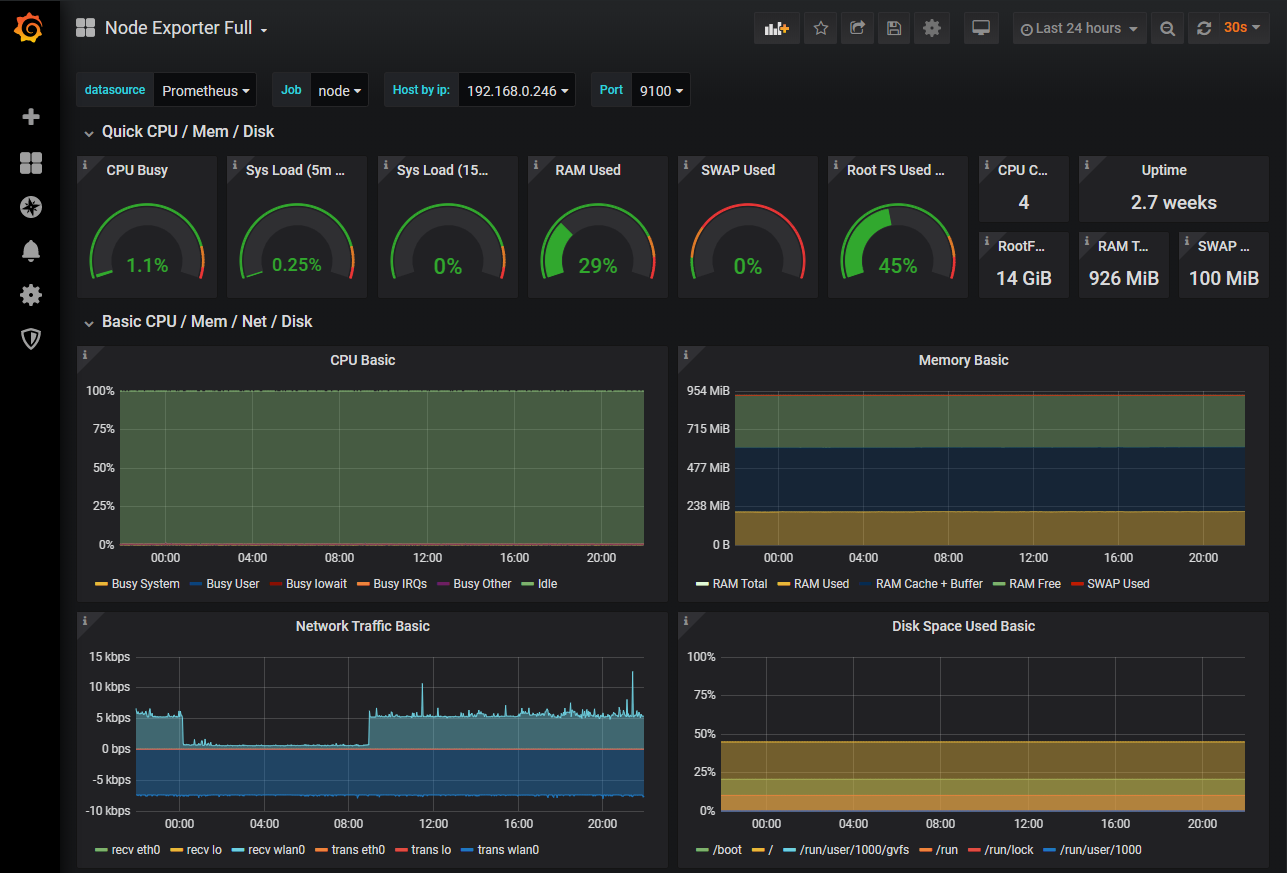
\includegraphics[width=\textwidth]{img/app/grafana_example.png}
  \caption{Exemple de visualisation des données exportées par \textit{node\_exporter} avec Grafana}
  \label{fig:grafnode}
\end{figure}


\begin{figure}
  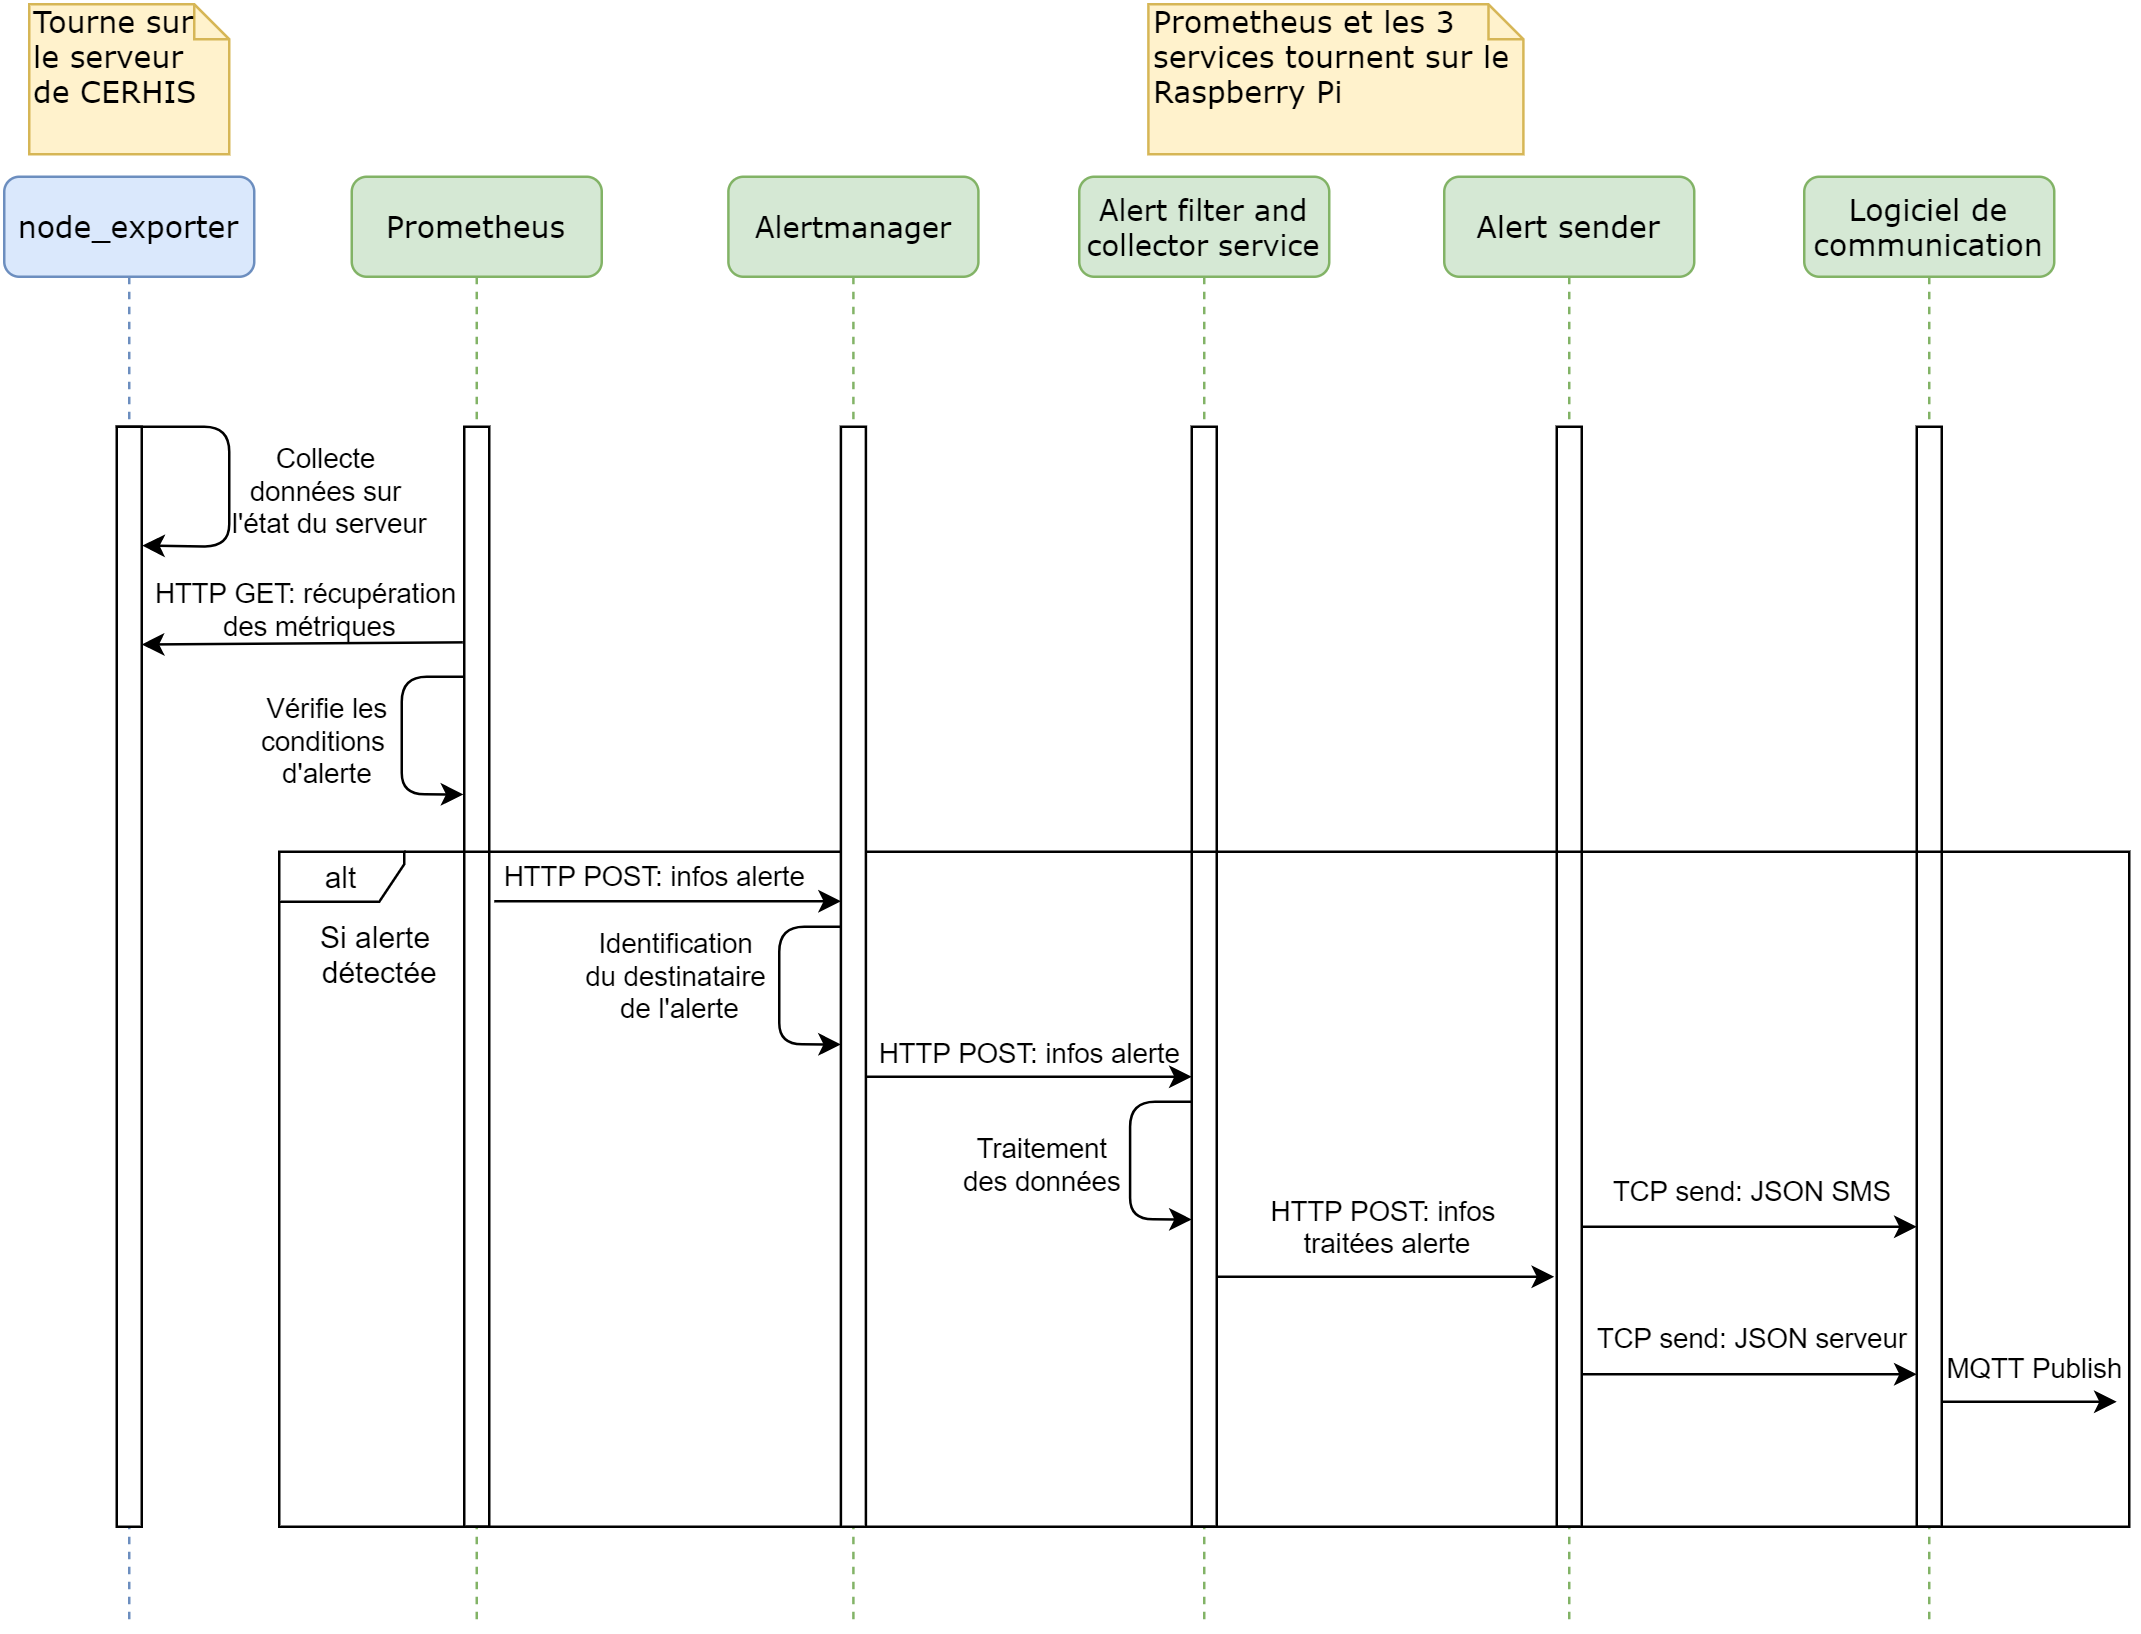
\includegraphics[width=\textwidth]{img/app/server_mon.png}
  \caption{Diagramme de séquence du processus de monitoring de l'état du serveur CERHIS. Ce processus est répété toutes les 15 secondes.
  Le MQTT publish a lieu comme décrit dans la section Envoi de données.}
  \label{fig:seqnodemon}
\end{figure}

~

\noindent
Cependant, l'utilisation de Prometheus apporte un nouveau problème au prototype. En effet, comme expliqué précédemment, la solution de communication utilise le protocole MQTT qui est basé sur le modèle publish-subscribe. En revanche, Prometheus utilise le protocole HTTP et le modèle \textit{pull} pour échanger des données. Cela complique énormément l'envoi de données et rend impossible l'utilisation de l'architecture de fédération de Prometheus. Par conséquent, lors de ce prototype, seulement l'envoi des alertes a été implémenté. Les alertes suivent un modèle \textit{push}, ce qui peut facilement être remplacé par un MQTT \textit{publish}.


\newpage
\subsubsection{Mappage du réseau local}

\noindent
Le mappage des dispositifs connectés au réseau est une étape essentielle avant de commencer à surveiller leur présence. Cette étape pourrait être remplacée par une configuration manuelle, mais cela a plusieurs désavantages. En effet, cela demanderait qu'un technicien encode manuellement toutes les adresses IP ou MAC des dispositifs connectés. Cela peut être une possible source d'erreur qui engendrait des problèmes lors du monitoring. En outre, la configuration devrait être modifiée à chaque fois qu'une nouvelle machine est ajoutée au réseau de CERHIS.

~

\noindent
Automatiser le processus de mappage permet donc de corriger ces problèmes. Grâce au protocole ARP\footnote{Address Resolution Protocol}, mapper le réseau est très facile. Ce protocole est généralement utilisé pour traduire des adresses de la couche réseau (IP) en adresses de la couche de liaison (MAC). La figure 1 montre un exemple sur le fonctionnement de ce protocole. Brièvement, un hôte \textit{broadcast} une requête ARP à travers le réseau local contenant une adresse IP. Si une machine de ce réseau s'est vu attribuer l'adresse IP incluse dans la requête, elle répond alors à l'hôte avec son adresse MAC. Les machines restantes reçoivent également la requête, mais comme leur adresse IP ne correspond pas, elles ignorent la demande. \footnote{ceci présume qu'aucune personne malveillante n'est connectée dans le réseau. Pour plus d'informations à ce sujet, vous pouvez effectuer des recherches sur l'ARP poisoning}

\begin{figure}[ht!]
  \centering
  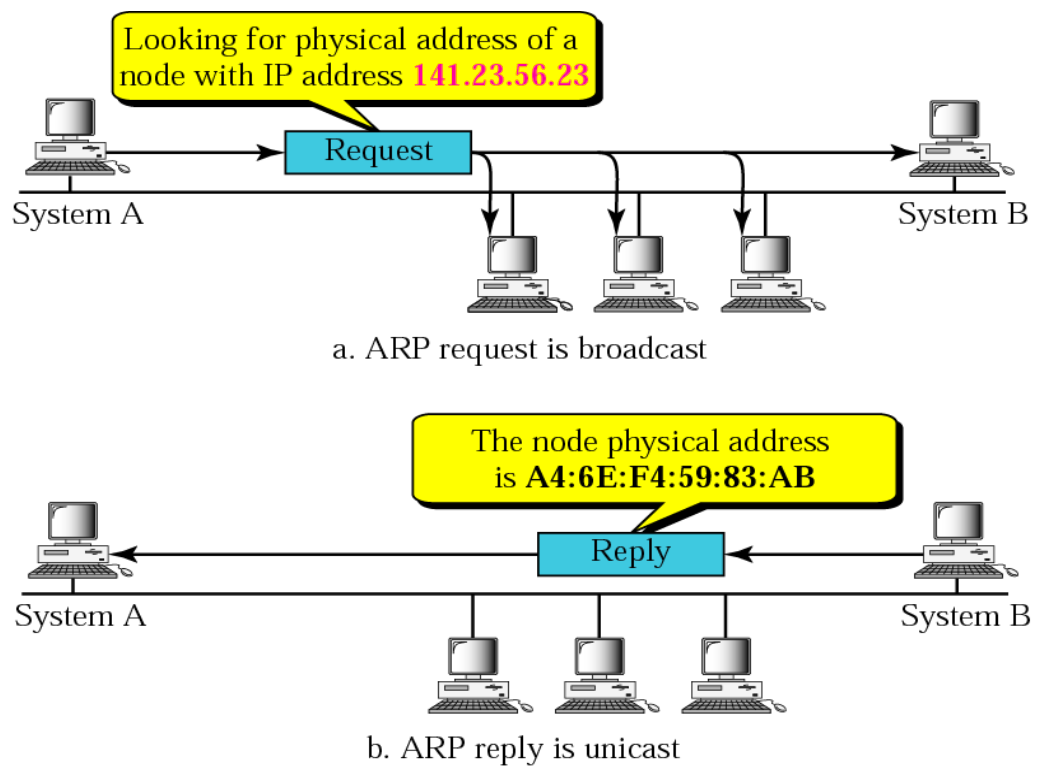
\includegraphics[width=0.7\textwidth]{img/app/arp.png}
  \caption{Exemple de fonctionnement du protocole ARP. Dans cet exemple, le système B possède l'adresse IP 141.23.56.23 \cite{arp_img}}
  \label{fig:arp_ex}
\end{figure}

~

\noindent
Afin de mapper le réseau, il suffit alors d'envoyer une requête ARP pour chaque adresse IP possible. Les dispositifs connectés répondront tous "présent" au moment où ils recevront une requête qui leur est destinée, permettant de réaliser le mappage assez rapidement.  Le logiciel NMAP a été employé car il est open source. L'application Fing \cite{fing_app} a été considéré comme une alternative, car elle est très efficace pour identifier le système d'exploitant des différentes machines connectées dans le réseau. Cependant, cette application est payante, d'où la raison pour laquelle elle n'a pas été choisie.

~

\noindent
La bibliothèque logicielle de NMAP sur Python a été exploitée pour interfacer avec le logiciel NMAP et traiter plus facilement le résultat du mappage. De plus, une base de données SQLite a été utilisée pour enregistrer la liste des dispositifs trouvés. La figure \ref{fig:db_device} affiche le diagramme de la table utilisé pour stocker les informations sur les dispositifs.

\begin{figure}[ht!]
  \centering
  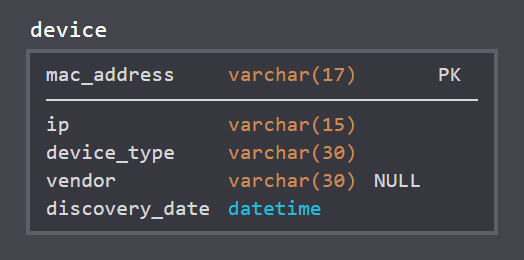
\includegraphics[width=0.45\textwidth]{img/app/device_db.png}
  \caption{Schéma de la table utilisée pour enregistrer les informations sur les dispositifs}
  \label{fig:db_device}
\end{figure}

~

\noindent
Comme expliqué plus tôt, le logiciel de monitoring est constitué de plusieurs services et le mappage correspond à l'un d'entre eux. Afin de rendre le résultat accessible aux services restants, une API REST a été implémentée en utilisant le web framework Flask. Ceci permet aux services qui nécessitent de la liste de dispositif de l'obtenir à partir d'une requête HTTP GET.

~

\noindent
Finalement, lorsque le service de mappage a été testé pour la première fois, il n'était pas capable d'identifier tous les dispositifs connectés sur le réseau. En particulier, cela semblait toujours se produire avec le même sous-ensemble d'appareils Android qui était connecté au réseau à travers le Wi-Fi. Ceci était un énorme problème puisque CERHIS possède des tablettes Android. Pour tenter de résoudre ce souci, la première proposition fut de réduire la périodicité de l'envoi des requêtes ARP. Ceci a permis de détecter quelques dispositifs supplémentaires, mais quelques smartphones continuaient à poser le même problème. La deuxième technique a été de suivre le chemin inverse. En effet, au lieu de diminuer la cadence, l'idée fut de réaliser plusieurs mappages consécutifs pour inonder le réseau avec plusieurs requêtes. Grâce à cette deuxième approche, tous les appareils ont pu être trouvés. Finalement, la solution implémentée est un hybride de ces deux techniques. Premièrement, un scan avec une très faible cadence est exécuté. Ensuite, trois mappages sont effectués en succession. Lors des tests réalisés, cette dernière solution s'est montrée $100\%$ efficace.

~

\noindent
Finalement, la décision a été prise de ne scanner le réseau qu'une seule fois lorsque le service est lancé. On peut s'attendre à ce que l'ensemble des appareils de CERHIS reste assez constant dans le temps. En outre, scanner le réseau en continu conduirait à deux situations difficiles à gérer qui sont :
\begin{itemize}
  \item En cas de disparition d'un appareil, il ne serait pas trouvé durant le scan plus récent. Quelle action devrait alors être adoptée dans cette situation ? Retirer le dispositif de la liste ou ignorer sa disparition ? Il est impossible de savoir exactement ce qui s'est passé et adapter un des deux comportements ne permettrait pas de résoudre entièrement le problème.

  ~

  \item Réaliser un balayage en continu rendrait la connexion temporaire d'appareils très difficile. En effet, un technicien pourra nécessiter de connecter son ordinateur ou smartphone pour accéder au serveur ou à l'interface de visualisation de données. Si un scan en continu est effectué, ce dispositif serait détecté et ajouté à liste d'appareils de CERHIS, même s'il n'en fait pas partie.

  ~

  \item 	Enfin, un balayage du réseau utilise une grande quantité de ressources sur la machine qui exécute le service, mais aussi sur les dispositifs du réseau puisque les trames (frames) sont broadcast.
\end{itemize}

~

\noindent
Si un appareil doit être ajouté ou retiré du réseau, il suffira alors de redémarrer manuellement le service et les modifications seront prises en compte assez rapidement.


\subsubsection{Surveiller la présence des divers composants}

\noindent
Une fois le mappage du réseau terminé, la liste des machines connectées peut être utilisée pour connaître les adresses IP et MAC des dispositifs à surveiller. Généralement, le protocole ICMP ECHO, aussi connu sous le nom de Ping, est employé afin de savoir si un dispositif est toujours connecté au réseau. Des requêtes d'ECHO (\textit{echo-request}) sont transmises par le dispositif désirant connaître s'il sait contacter l'appareil destinataire. Ensuite, le destinataire reçoit la demande et envoie une réponse echo (\textit{echo-reply}) à l'émetteur. Ce procédé est résumé sur la figure \ref{fig:icmp}.


\begin{figure}[ht!]
  \centering
  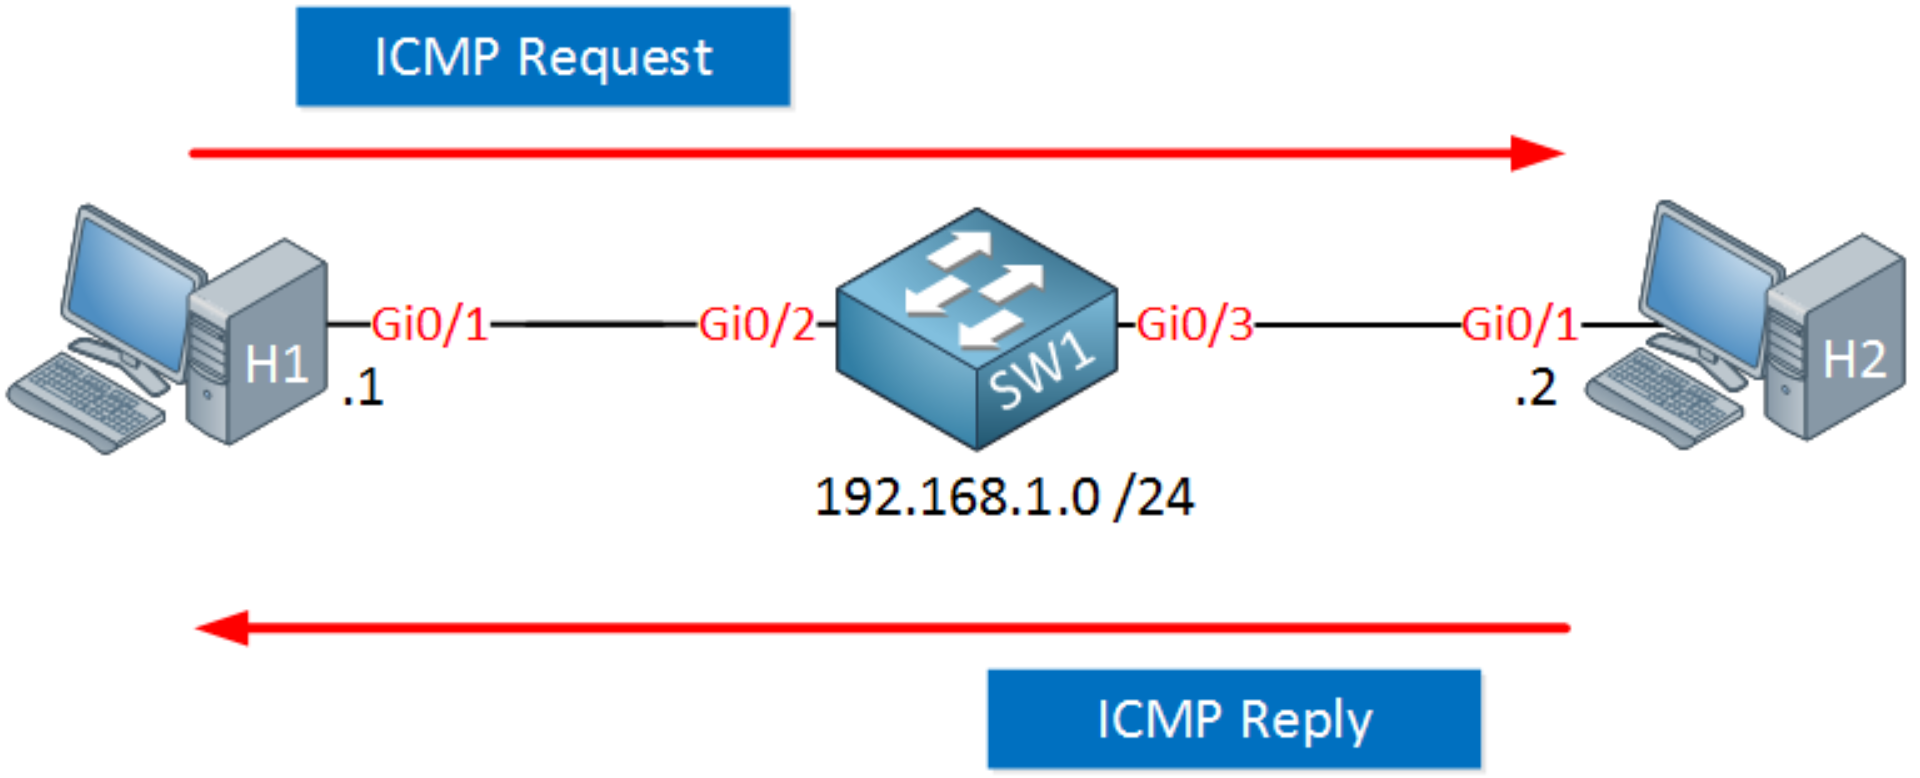
\includegraphics[width=0.60\textwidth]{img/app/ping.png}
  \caption{Exemple d'un Ping (ICMP \textit{echo-request} et ICMP \textit{echo-reply})}
  \label{fig:icmp}
\end{figure}


~

\noindent
Cependant, de nombreux pare-feux bloquent ce type de trafic, ce qui rend impossible de connaître si l'appareil est connecté au réseau. En revanche, le protocole ARP n'est presque jamais bloqué, car il est nécessaire afin que les dispositifs puissent communiquer. Mais, comme mentionné ci-dessus, les demandes ARP sont broadcast à travers tout le réseau, ce qui peut générer beaucoup de trafic et avoir un impact sur les performances de ce dernier. De ce fait, dans un premier temps, NMAP a été employé pour monitorer les appareils. Cela permettrait de laisser le logiciel choisir la méthode idéale pour surveiller chaque dispositif.

~

\noindent
Cette implémentation s'est avérée très efficace à détecter si un appareil était connecté. Au contraire, elle ne s'est pas montrée aussi fonctionnelle du point de vue de l'utilisation des ressources, créant des pics d'utilisation du CPU de l'ordre de $60\%$. Sachant que les pings doivent être effectués assez fréquemment, cette méthode a dû être abandonnée. En effet, une utilisation élevée du processeur aurait entraîné une haute consommation d'énergie, ce qui aurait engendré des problèmes lorsque l'appareil serait alimenté par une batterie.

~

\noindent
La bibliothèque logicielle scapy a été manipulée par la suite pour concevoir une solution plus adaptée au contexte de ce projet. Scapy permet de générer manuellement des paquets et des trames de plusieurs protocoles. Puisque les adresses IP et MAC sont connues (grâce au scan), il est alors très facile de créer un paquet ICMP et de l'encapsuler par une trame qui contient l'adresse MAC du destinataire. Ceci retire la responsabilité au système d'exploitation de créer la trame et optimise tout le processus. En effet, si jamais la MAC ne se trouve pas dans la table ARP, le système d'exploitation doit broadcast une requête ARP. Ajouter manuellement l'adresse MAC évite ce broadcast.

~

\noindent
Cette méthode fonctionne avec la majorité des dispositifs, mais ne résout pas le problème lorsque le pare-feu de l'appareil filtre les paquets ICMP. De ce fait, si un dispositif ne répond pas à une demande d'ECHO après 2 secondes, une requête ARP contenant l'adresse IP de ce dispositif est broadcast dans le réseau. La combinaison de ces deux procédés permet d'avoir un taux de succès très élevé. Cependant, même en recourant à ces deux techniques, il est arrivé que certains smartphones Android ne répondissent à aucune des demandes. Ce comportement était assez rare, mais avait tout de même un impact sur la qualité de la solution. Pour le résoudre, une approche assez similaire à celle du mappage du réseau a été utilisée. Lorsque l'appareil ne réagit à aucune des deux requêtes précédentes, de multiples paquets ICMP sont envoyés en succession pendant une période de 4 secondes. Ces paquets sont également encapsulés dans une trame qui contient l'adresse MAC du destinataire. Enfin, la combinaison de ces trois techniques a permis d'atteindre une très haute bonne détection de la présence des dispositifs. De plus, il n'a pas été possible de reproduire le même problème avec les smartphones Android lorsque les 3 techniques sont utilisées. Un diagramme de flux du processus de monitoring est présenté dans la figure \ref{fig:device_presence}.

\begin{figure}[ht!]
  \centering
  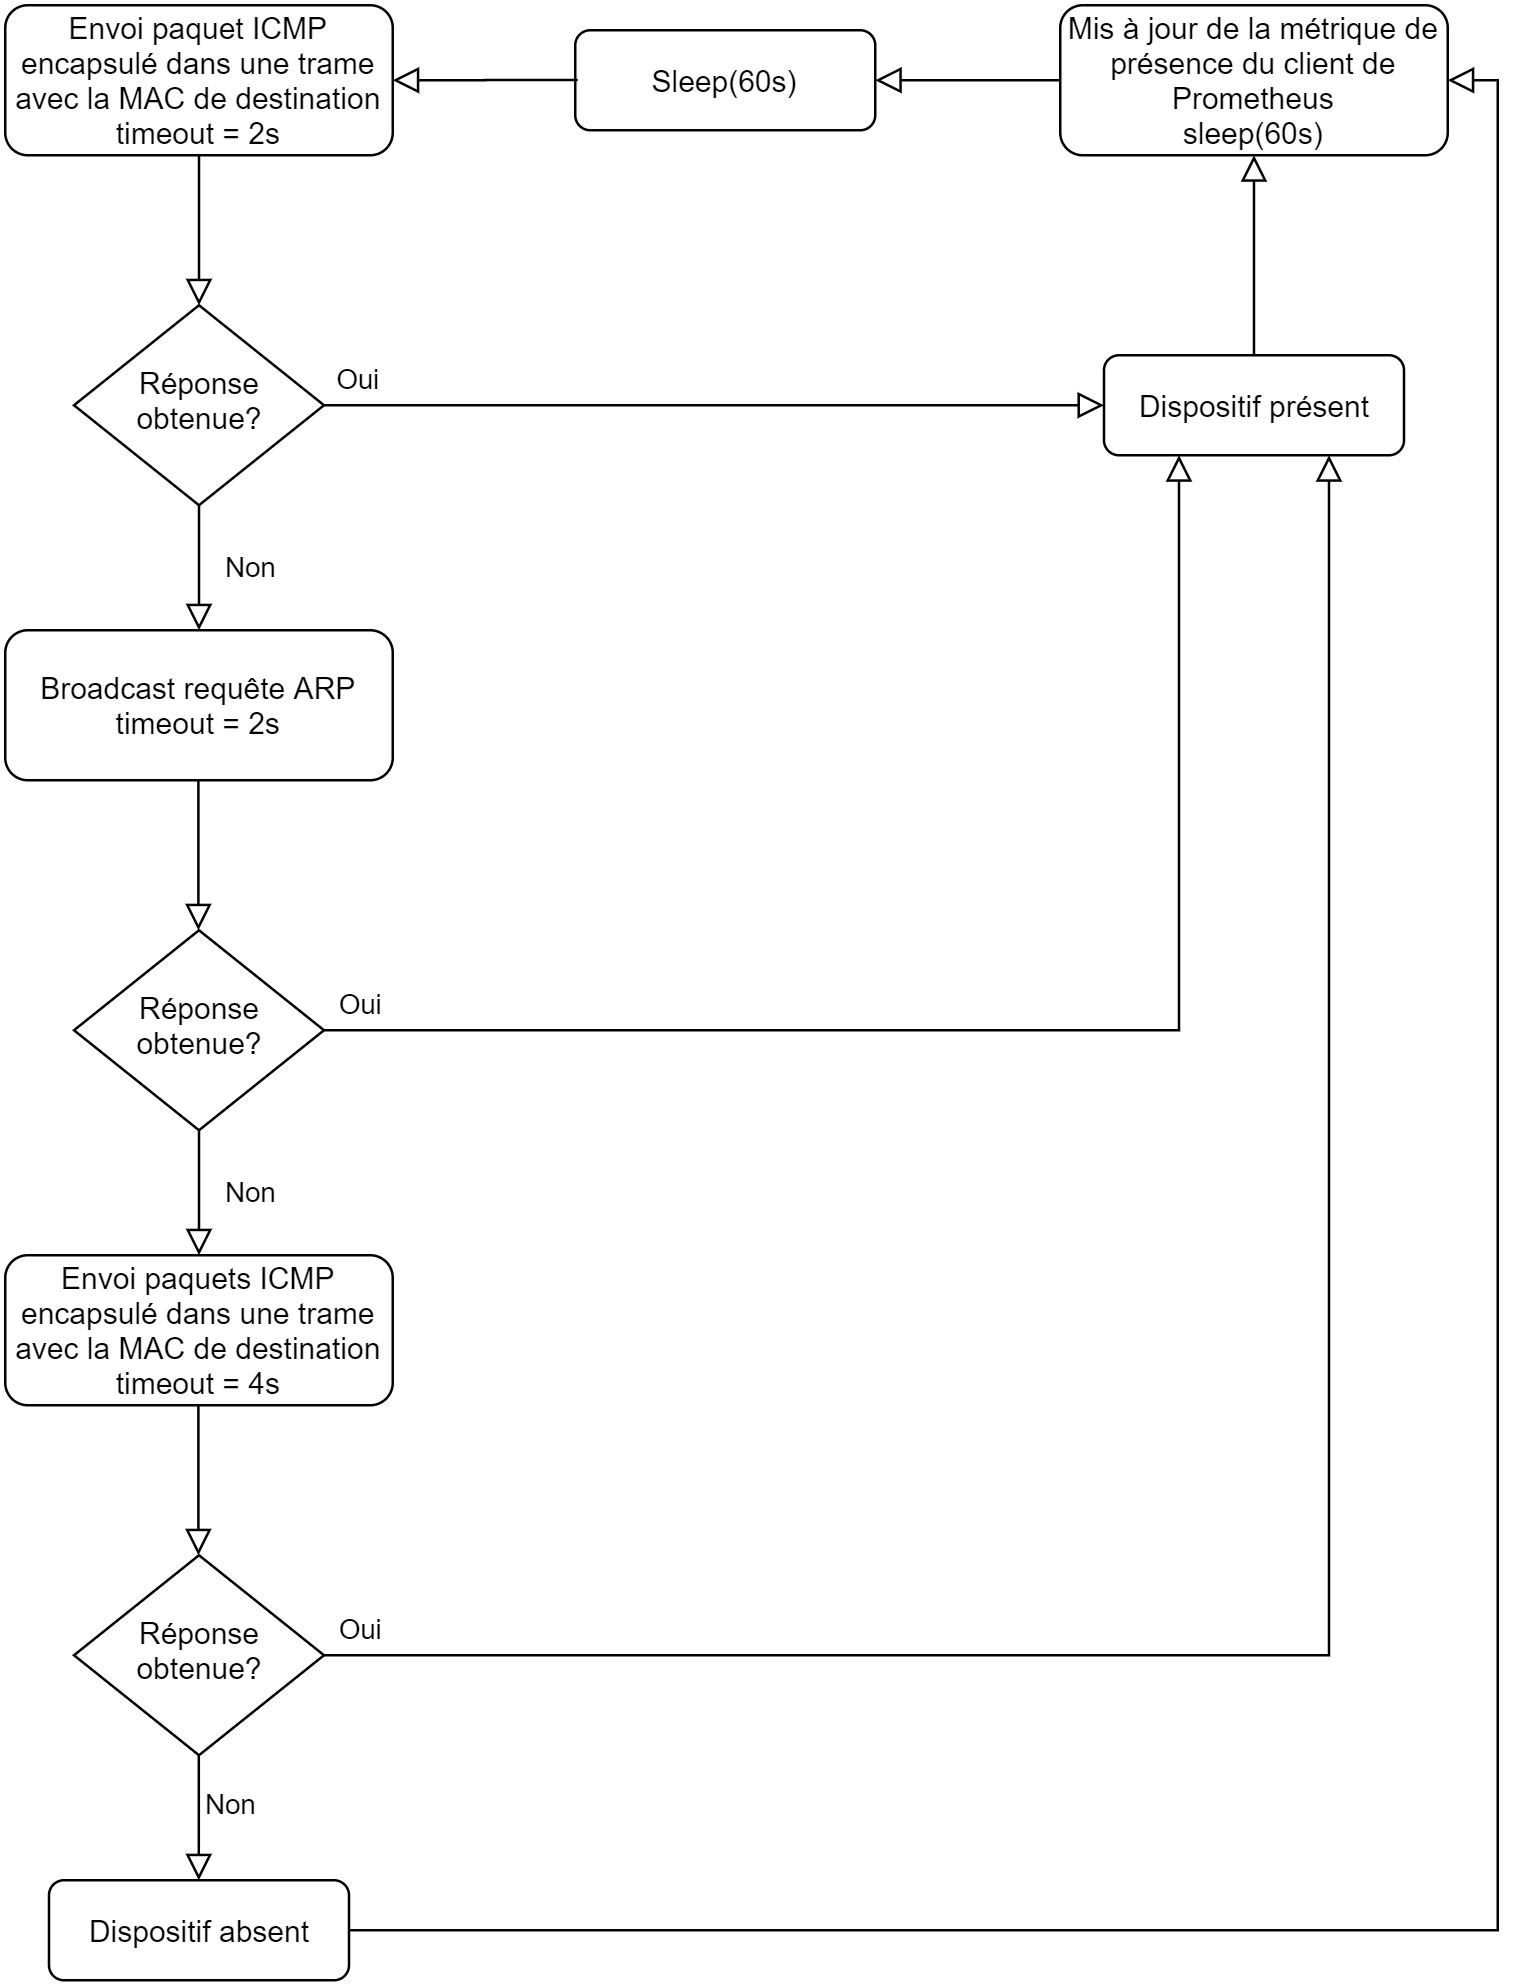
\includegraphics[width=0.68\textwidth]{img/app/device_mon.png}
  \caption{Diagramme de flux du processus de vérification de la présence d'un dispositif}
  \label{fig:device_presence}
\end{figure}
~

\noindent
Finalement, il fallait implémenter la sauvegarde des données de présence et produire les alertes en cas de disparition d'un appareil. Cela aurait pu être développé manuellement. Mais, puisque Prometheus était déjà déployé comme base de données et gestionnaire d'alertes, l'utiliser également pour stocker les informations sur la présence des appareils semblait être la solution plus naturelle. En outre, cela permet aussi d'exploiter toutes les capacités de gestion d'alertes pour configurer et générer des messages lorsqu'un dispositif est manquant. Pour exporter les données de présence, le client Prometheus pour Python a été utilisé. L'architecture finale de la solution de surveillance est exposée dans la figure \ref{fig:arch_final}.


\begin{figure}[ht!]
  \centering
  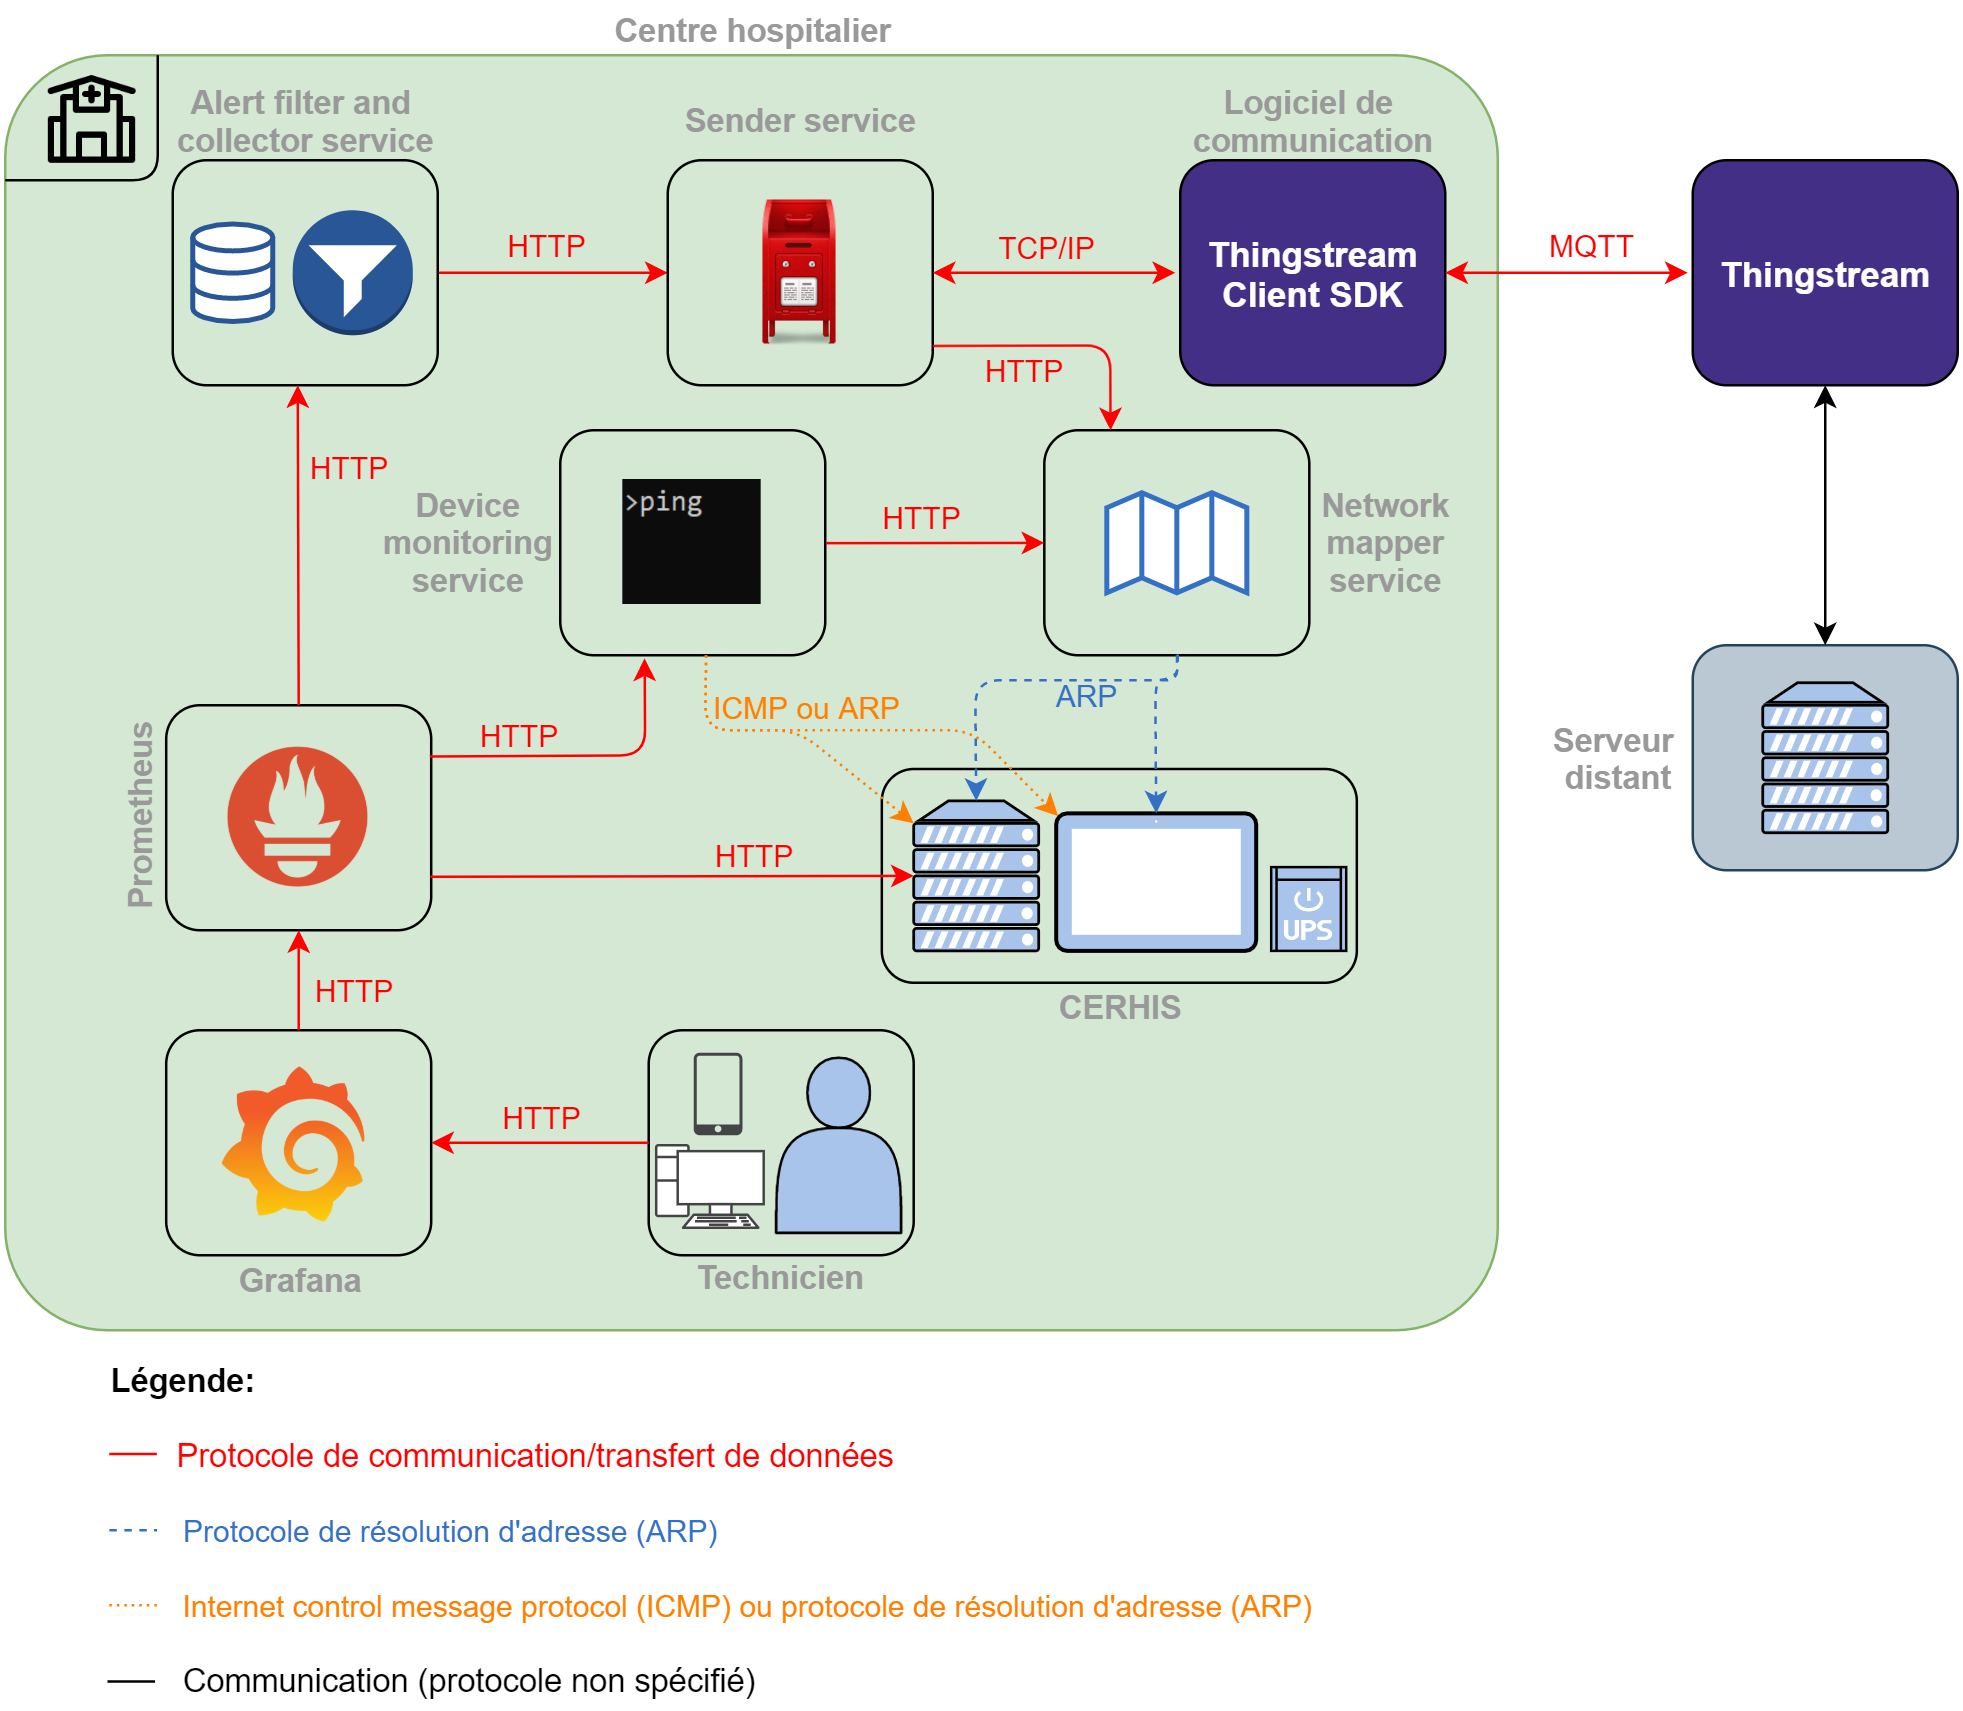
\includegraphics[width=\textwidth]{img/app/arch_complete.png}
  \caption{Architecture complète du client de monitoring}
  \label{fig:arch_final}
\end{figure}


~

\newpage

\noindent
Maintenant que l'entièreté de la solution de monitoring a été présentée, il est possible de revenir sur quelques détails qui ont été omis sur les sections antérieures pour faciliter les explications. Premièrement, la configuration actuelle de Prometheus permet d'identifier et envoyer des messages pour quatre types d'alertes qui sont :

\begin{itemize}
  \item \textbf{ServerRestart} : Cette alerte emploie les données exportées par le \textit{node\_exporter} afin de repérer si le serveur a redémarré au cours des 10 dernières minutes.

  ~

  \item \textbf{Process Down} : Détecte si un des processus surveillés par le service \textit{process-exporter} a été interrompu. La liste des process monitorés est définie dans le fichier de configuration de \textit{process-exporter}.

  ~

  \item \textbf{DeviceDown} : Exploite les données relatives à la présence des dispositifs exportées par le service device monitoring pour vérifier si un appareil est absent depuis plus de 2 minutes.

    ~

  \item \textbf{InstanceDown} : Cette alerte a lieu si un des services \textit{exporters} utilisés par Prometheus pour obtenir les données cesse de répondre aux requêtes HTTP.
\end{itemize}

~

\noindent
Ces quatre alertes correspondent à ce qui était initialement demandé dans le cahier des charges. À l'avenir, d'autres alertes pourront être ajoutées par le biais des fichiers de configuration de Prometheus, comme celui illustré dans le listing \ref{lst:alert}.

~

\noindent
Deuxièmement, le \textit{sender service} ne se limite pas à transférer les alertes envoyées par le logiciel \textit{alert filter and collector}. En effet, lors de son initialisation, le \textit{sender service} essaye de contacter le \textit{network mapper} afin d'obtenir la liste de dispositifs. Cette liste est ensuite transmise au service de communication qui l'envoie au serveur.

~

\noindent
Enfin, l'\textit{alert filter and collector service} emploie une base de données SQLite afin de sauvegarder de façon permanente toutes les alertes générées par Prometheus. En cas de défaillance de la solution de communication, les techniciens pourront récupérer le fichier de la base de données et avoir accès à un historique des événements, même plusieurs jours après qu'ils se soient produits. Le schéma de la base de données est illustré dans la figure \ref{fig:alert_db}.


\begin{figure}[ht!]
  \centering
  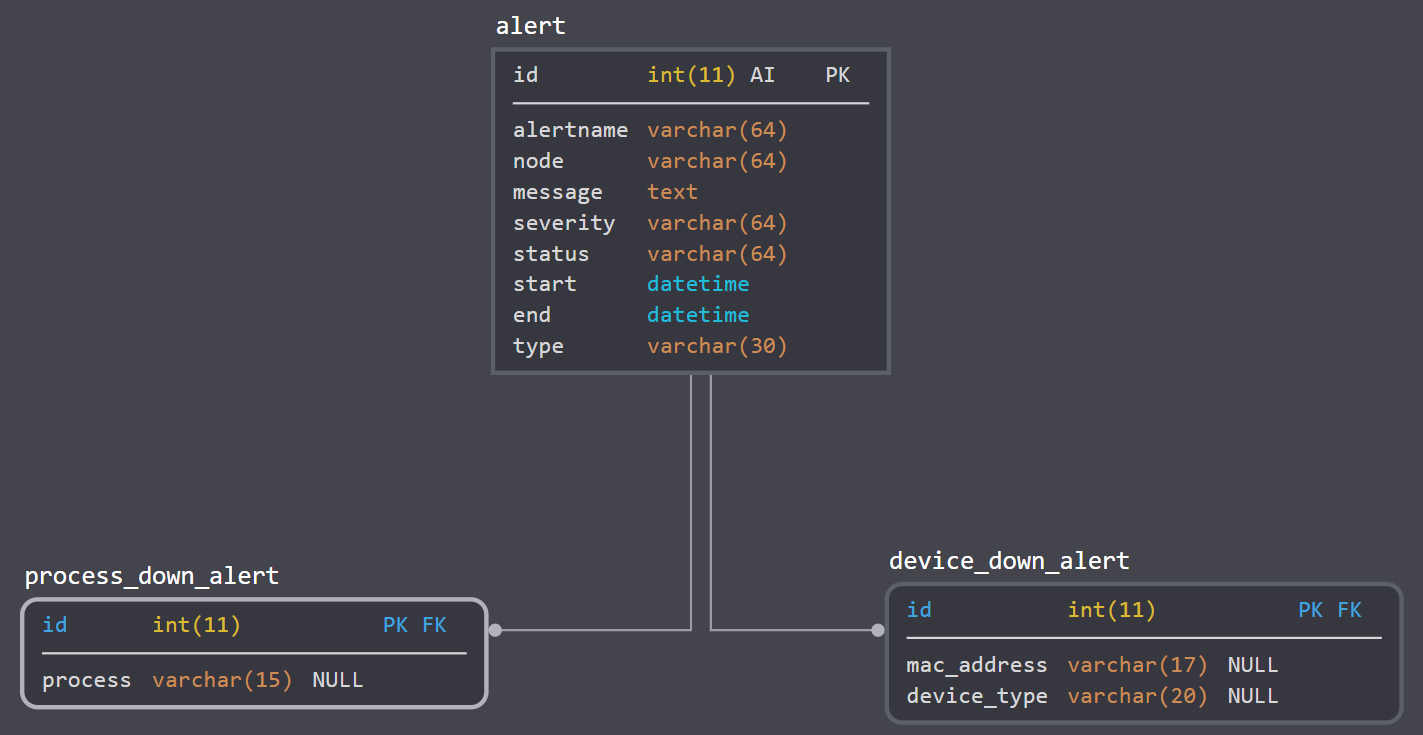
\includegraphics[width=0.85\textwidth]{img/app/alert_db.png}
  \caption{Schéma de la base de données du \textit{alert filter and collector service}}
  \label{fig:alert_db}
\end{figure}

\newpage
\subsection{Sécurité}

\noindent
La sécurité ne figurait pas parmi les objectifs du cahier des charges, d'où la raison pour laquelle elle n'a pas vraiment été prise en compte lors de la réalisation de ce prototype. En fait, les hypothèses suivantes ont été faites :

\begin{itemize}
  \item Aucun agent malveillant n'est connecté au réseau local de CERHIS.

  ~

  \item Aucun dispositif malveillant ne peut se connecter au réseau de Thingstream. En particulier, aucun agent malveillant ne pourra se faire passer par un client SN-Thing.
\end{itemize}

~

\noindent
Cette dernière hypothèse se traduit donc par une confiance totale dans le système d'authentification de la carte SIM de Thingstream et du réseau GSM. Cependant, dans une version finale du client, faire cette hypothèse ne serait peut-être pas judicieux. Il est fortement recommandé qu'une technique d'échange de clés soit implémentée entre le serveur et le client de communication afin que les transmissions entre les deux instances puissent être cryptées. Ceci empêcherait donc d'être complètement du système de sécurité de Thingstream qui nous est inconnu. En outre, le chiffrement des données permettrait d'être protégé contre des attaques sur le réseau GSM. Ces attaques ne sont pas faciles à conduire, mais peuvent potentiellement exposer les informations transmises dans le réseau. \cite{gsm_fails}

\section{Serveur}
\label{sec:server}

\noindent
Le serveur distant est une partie intégrale de la solution finale. Il permet aux techniciens de consulter l'état actuel de l'infrastructure même s'ils ne se trouvent pas dans le centre hospitalier. Les SMS ne sont utilisés que pour les prévenir en cas de défaillance d'un des composants de CERHIS. Cependant, certaines de ces défaillances peuvent être de courte durée, voire même un faux positif. En outre, les SMS n'offrent pas une vue d'ensemble sur la liste des composants et l'historique des alertes. Le serveur cherche donc à surmonter ces problèmes en sauvegardant toutes les informations sur une longue période et en proposant un accès facile aux données à travers une interface graphique. Les informations sur le serveur seront également mises à jour en cas de changement, mais cela ne se fera pas par SMS.

~

\noindent
L'application s'exécutant sur le serveur est beaucoup plus simple que celle du client. En effet, le serveur ne fait que : recevoir des informations déjà traitées par ce dernier, les stocker sur la base de données et les rendre accessibles aux techniciens. De ce fait, l'architecture du logiciel est composée par les trois parties suivantes :


\begin{itemize}
  \item Le client MQTT, ou Thingstream IP-Thing, qui reçoit tous les messages publiés sur les topics \textbf{device/\#identity\#/startup} et \textbf{device/\#identity\#/post}.

  ~

  \item Une base de données capable de stocker toutes les informations envoyées par plusieurs clients.

  ~

  \item Une application ou un service permettant de facilement visualiser les données se trouvant sur la base de données.
\end{itemize}

~

\noindent
La figure \ref{fig:base_server} illustre cette architecture. L'implémentation de chaque composant sera exposée au cours des trois sections suivantes.

\begin{figure}[ht!]
  \centering
  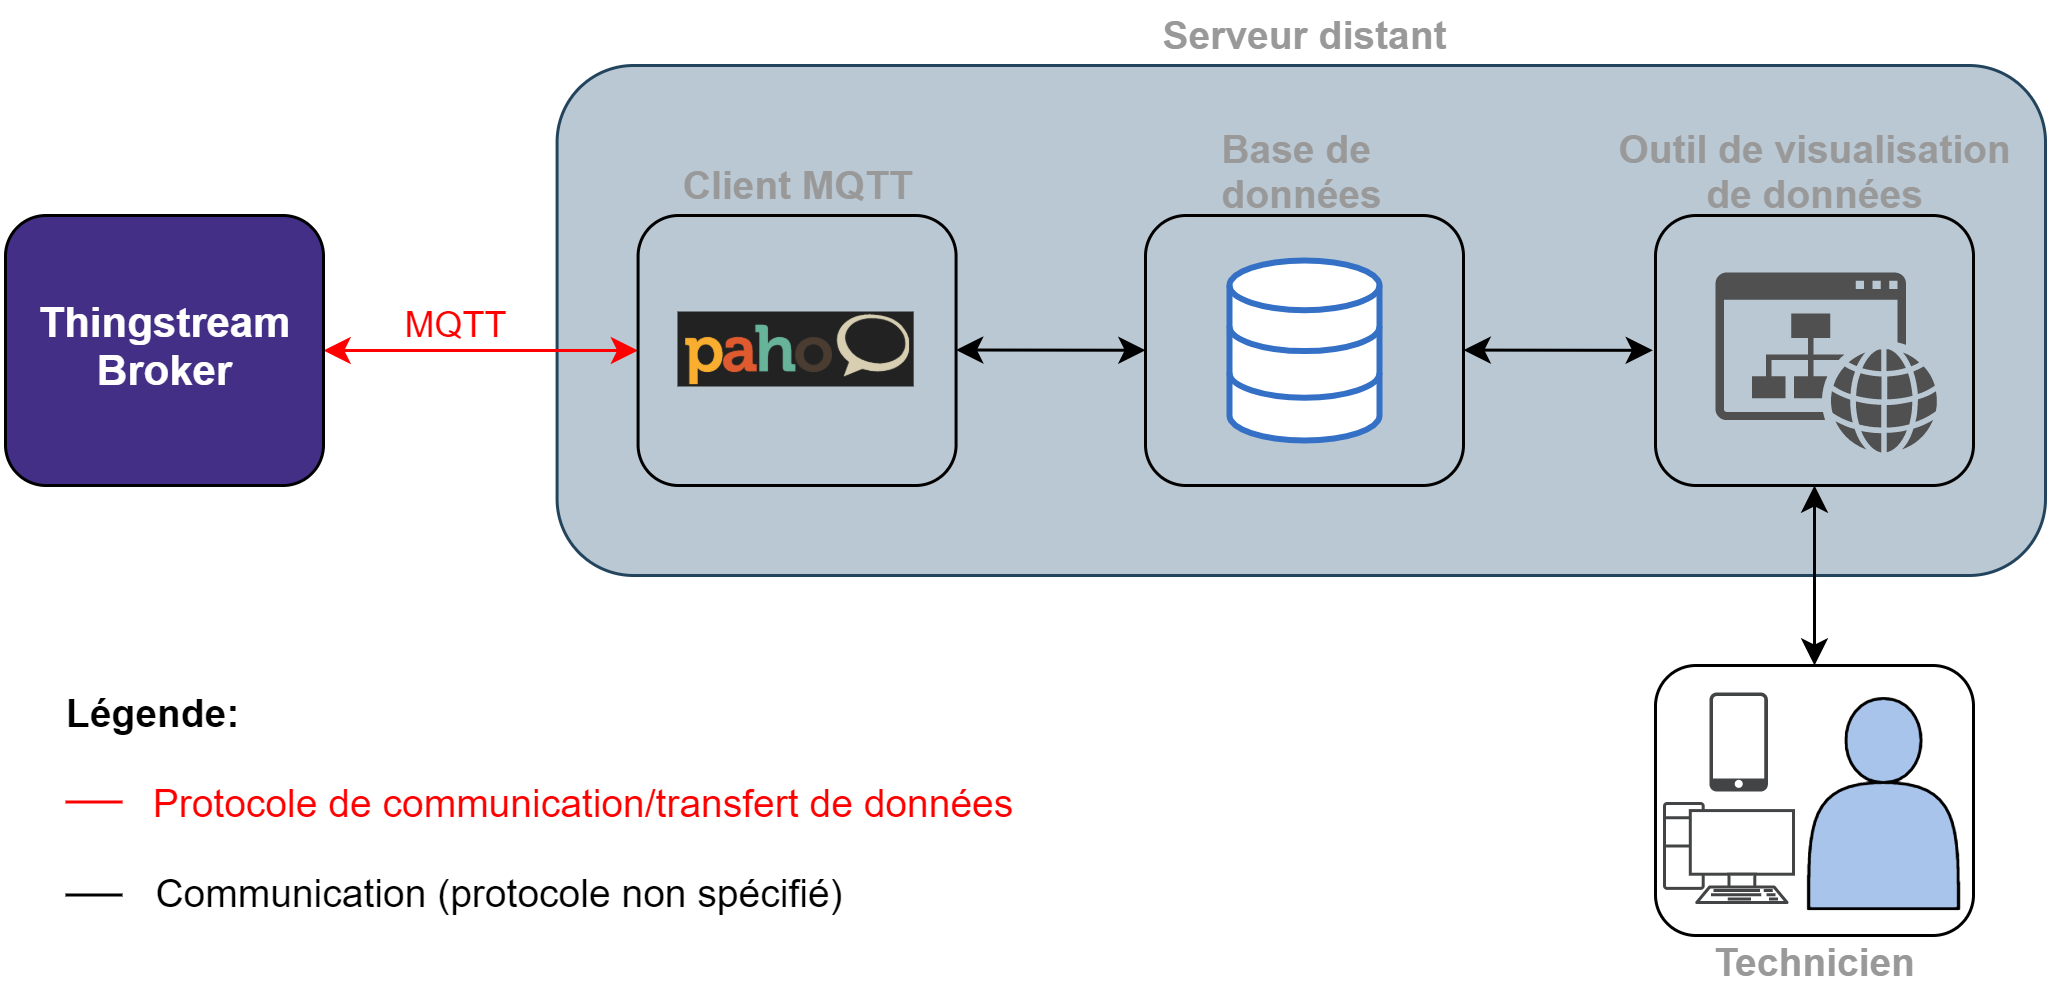
\includegraphics[width=\textwidth]{img/app/base_server.png}
  \caption{Architecture simplifiée de l'application tournant sur le serveur distant}
  \label{fig:base_server}
\end{figure}


\subsection{Base de données}

\noindent
De nos jours, plusieurs types de bases de données existent sur le marché, mais elles sont très souvent classées selon deux modèles : le modèle relationnel et les bases de données NoSQL (non relationnelles). Ces dernières abandonnent les propriétés ACID\footnote{atomicité, cohérence, isolation et durabilité} en faveur d'une plus haute disponibilité, de bonnes performances même lorsqu'une grande quantité de données doit être traitée, et l'extensibilité\footnote{\textit{scalability} en anglais}.

~

\noindent
Cependant, en raison des limitations de la solution de communication, seulement des mises à jour concernant l'état des alertes et la liste des dispositifs seront envoyées au serveur. Les métriques collectées par Prometheus ne seront stockées que sur le Raspberry Pi. Cet aspect a une grande influence sur le choix de la base de données. En effet, ceci diminue très fortement la quantité de données que le serveur devra enregistrer. En outre, toutes les informations envoyées par le client sont également stockées sur celui-ci sur des bases de données SQLite. Cela veut donc dire que les données transmises sont déjà formatées selon le modèle relationnel. Il apparaît tout à fait évident que la base de données du serveur suive le même modèle, puisque cela réduit le nombre de technologies à maitriser pour travailler sur ce projet.

~

\noindent
Le schéma de la base de données du serveur peut donc être très similaire à ceux présentés sur les figures \ref{fig:db_device} et \ref{fig:alert_db}. La grande différence c'est que les diverses tables peuvent être combinées sous un même schéma. Une base de données SQLite pourrait également être utilisée du côté du serveur, mais cela présenterait énormément de problèmes plus tard lorsque celui-ci recevrait des informations de multiples clients. SQLite a une très faible extensibilité et est optimisé pour les petites bases de données. Cependant, la base de données du serveur doit pouvoir stocker les informations de plusieurs clients. Le choix de SQLite n'est donc pas le plus judicieux pour ce projet.

~

\noindent
Il existe sur le marché des alternatives qui sont également open source et plus puissantes que SQLite. Contrairement à cette dernière, ces bases de données ne sont pas autonomes, elles ont besoin d'un \underline{serveur}\footnote{Ce serveur peut correspondre à la même machine du serveur distant ou à une seconde machine complètement différente. Jusqu'à présent, le mot serveur a été utilisé pour désigner l'ensemble constitué par le client MQTT, la base de données et la visualisation de données. En revanche, lors de la communication entre ces composants, certains jouent le rôle de client et d'autres celui du serveur. Par exemple, la solution de visualisation de données est un client qui se connecte au serveur de la base de données. Désormais, si les mots serveur et client sont soulignés, alors ils correspondent à ce dernier cas et non pas aux solutions créées dans ce mémoire.} pour fonctionner. Elles suivent donc le modèle \underline{client-serveur} pour échanger des données. Les 3 principales alternatives sont :

\begin{itemize}
  \item MySQL
  \item PostgreSQL
  \item MariaDB
\end{itemize}

~

\noindent
N'importe laquelle des trois possibilités aurait pu être déployée. Ce projet ne possède pas beaucoup de contraintes sur cet aspect et la structure des données à stocker n'est pas complexe. MySQL a été choisi parque que c'est une des plus répandues et, traditionnellement, celle qui est employée quand quelqu'un désire apprendre à manipuler des bases de données. En outre, puisque son utilisation est très habituelle, une grande majorité des outils de visualisation sont compatibles avec ce choix. Ce dernier aspect sera important plus tard lors de la définition de l'outil de visualisation de données.

~

\noindent
Afin de communiquer avec la base de données, la bibliothèque logicielle SQLAlchemy a été manipulée. Elle permet de faire abstraction de toute la partie liée aux requêtes SQL. Cela a contribué à réduire le temps de développement et à diminuer la complexité du code. Le schéma de la base de données du serveur distant est illustré dans \ref{fig:server_db_schema}. Veuillez noter l'ajout du \textit{thingstream\_id} dans chaque table, ce qui permet de différencier les données en fonction du centre hospitalier. En outre, la table \textit{thingstream\_device} a également été additionnée pour enregistrer les valeurs liées à la vérification de l'identité d'une application.


\begin{figure}[ht!]
  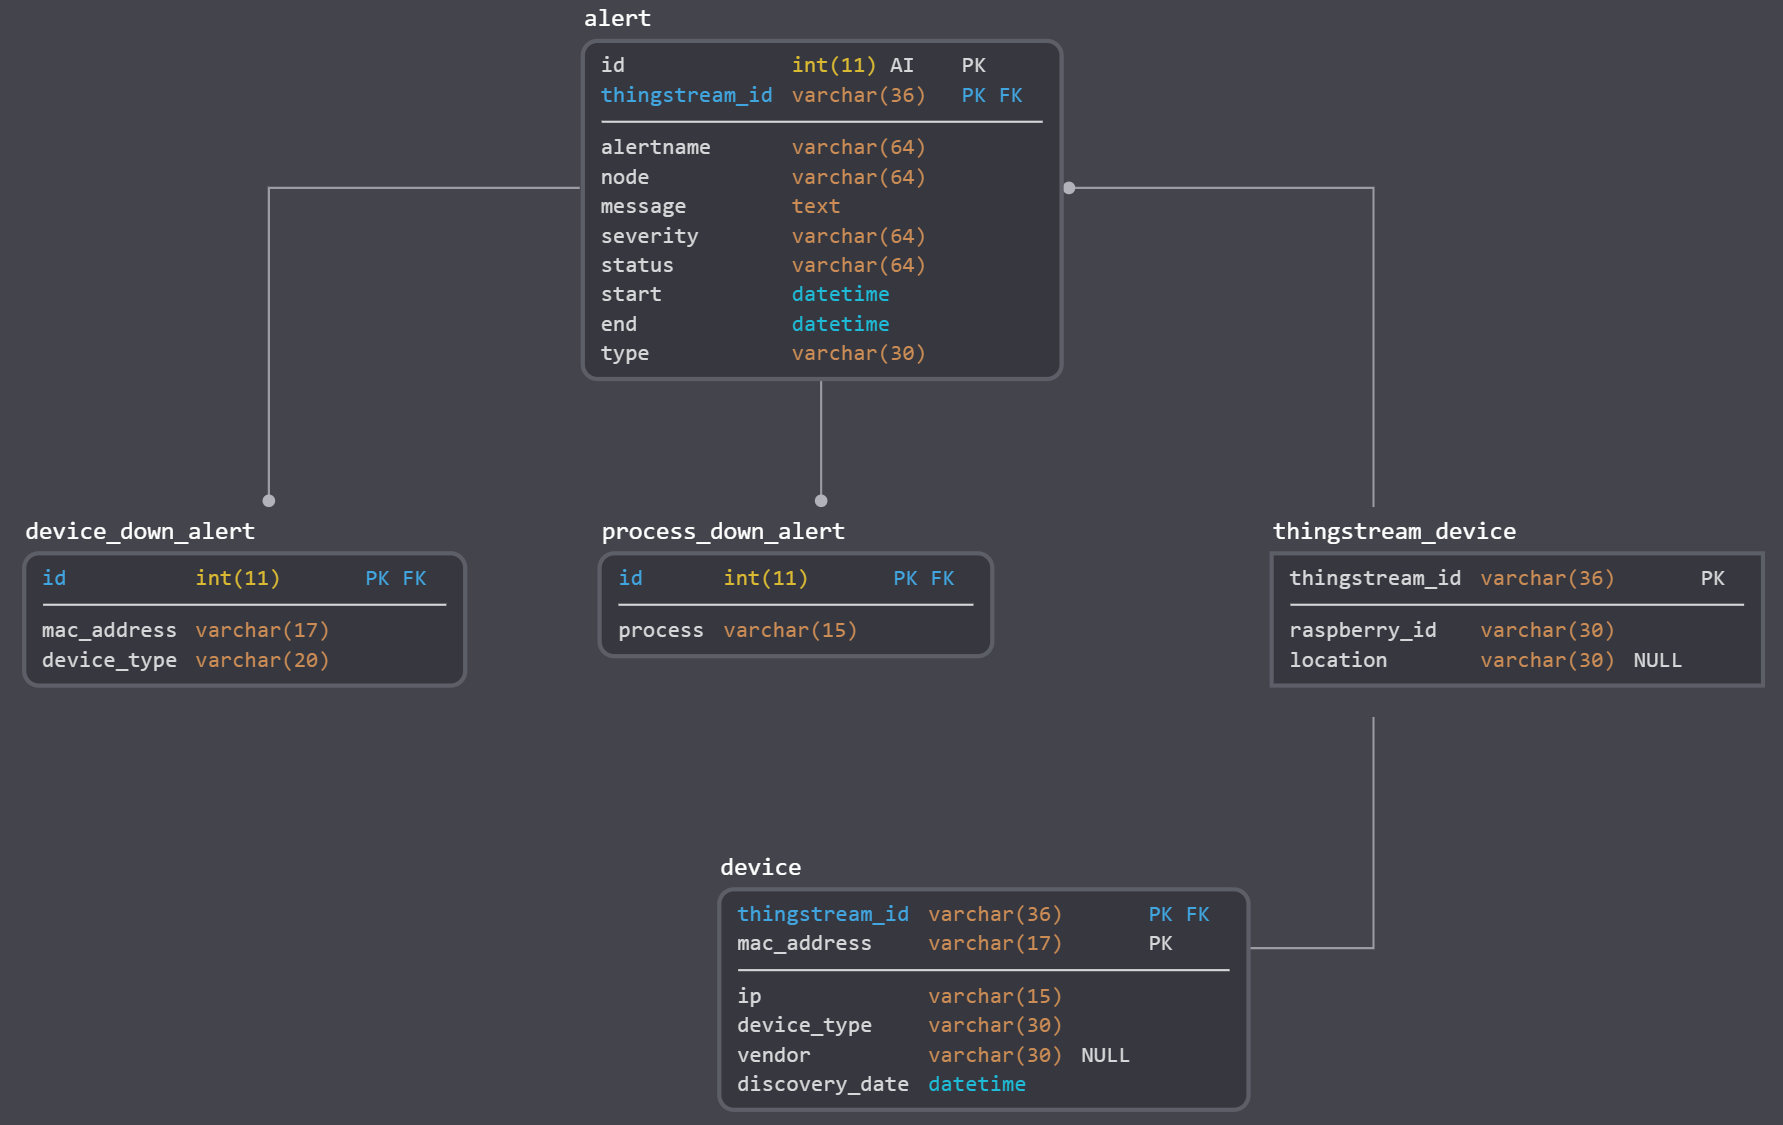
\includegraphics[width=\textwidth]{img/app/db_final.png}
  \caption{Schéma de la base de données du serveur}
  \label{fig:server_db_schema}
\end{figure}


\subsection{Implémentation des fonctionnalités}

\subsubsection{Client MQTT}

\noindent
Tout comme la base de données, le logiciel du serveur est assez simple. La bibliothèque logiciel Python Eclipse Paho MQTT a été utilisé pour implémenter le client qui reçoit tous les messages publiés par les SN-Things. Cette bibliothèque possède énormément de documentation et d'exemples d'utilisation en ligne.

~

\noindent
Comme expliqué au début de cette section, ce client est abonné à deux topics. Le premier, \textbf{device/\#identity\#/startup}, est le topic utilisé par les SN-Things lorsqu'une application essaye de s'authentifier auprès du serveur. Afin de vérifier l'identité, le serveur compare l'id envoyé par l'application et la valeur \textbf{\#identity\#} avec des valeurs encodées au préalable sur la base de données. En cas de correspondance (non-correspondance), le serveur répond avec un message autorisant (refusant) la demande de connexion de l'application. Ce message est lu par le client de communication tournant sur le Raspberry Pi qui, en fonction de la réponse, décidera ensuite de maintenir ou fermer la connexion avec l'application .

~

\noindent
Le deuxième, \textbf{device/\#identity\#/post}, correspond au topic employé pour transmettre les données relatives aux alertes et aux dispositifs. Dans ce cas, le serveur lit d'abord le type des données et ensuite enregistre les sur la table de la base de données qui correspondant au type présent dans l'en-tête.

~

\noindent
Afin de s'adresser à un SN-Thing en particulier, le serveur publie des messages sur le topic \textbf{device/\#identity\#/recv}. Actuellement, seulement le message d'acceptation ou de refus de la connexion est transmis. Ce message prend la forme suivante :

\begin{lstlisting}[language=json]
{
  "id" : #id#,
  "accepted" : #valeur booleenne#
}
\end{lstlisting}

~

\noindent
Finalement, la figure \ref{fig:auth_app_server} illustre le processus lié à la vérification de l'identité d'une application.

\begin{figure}[ht!]
  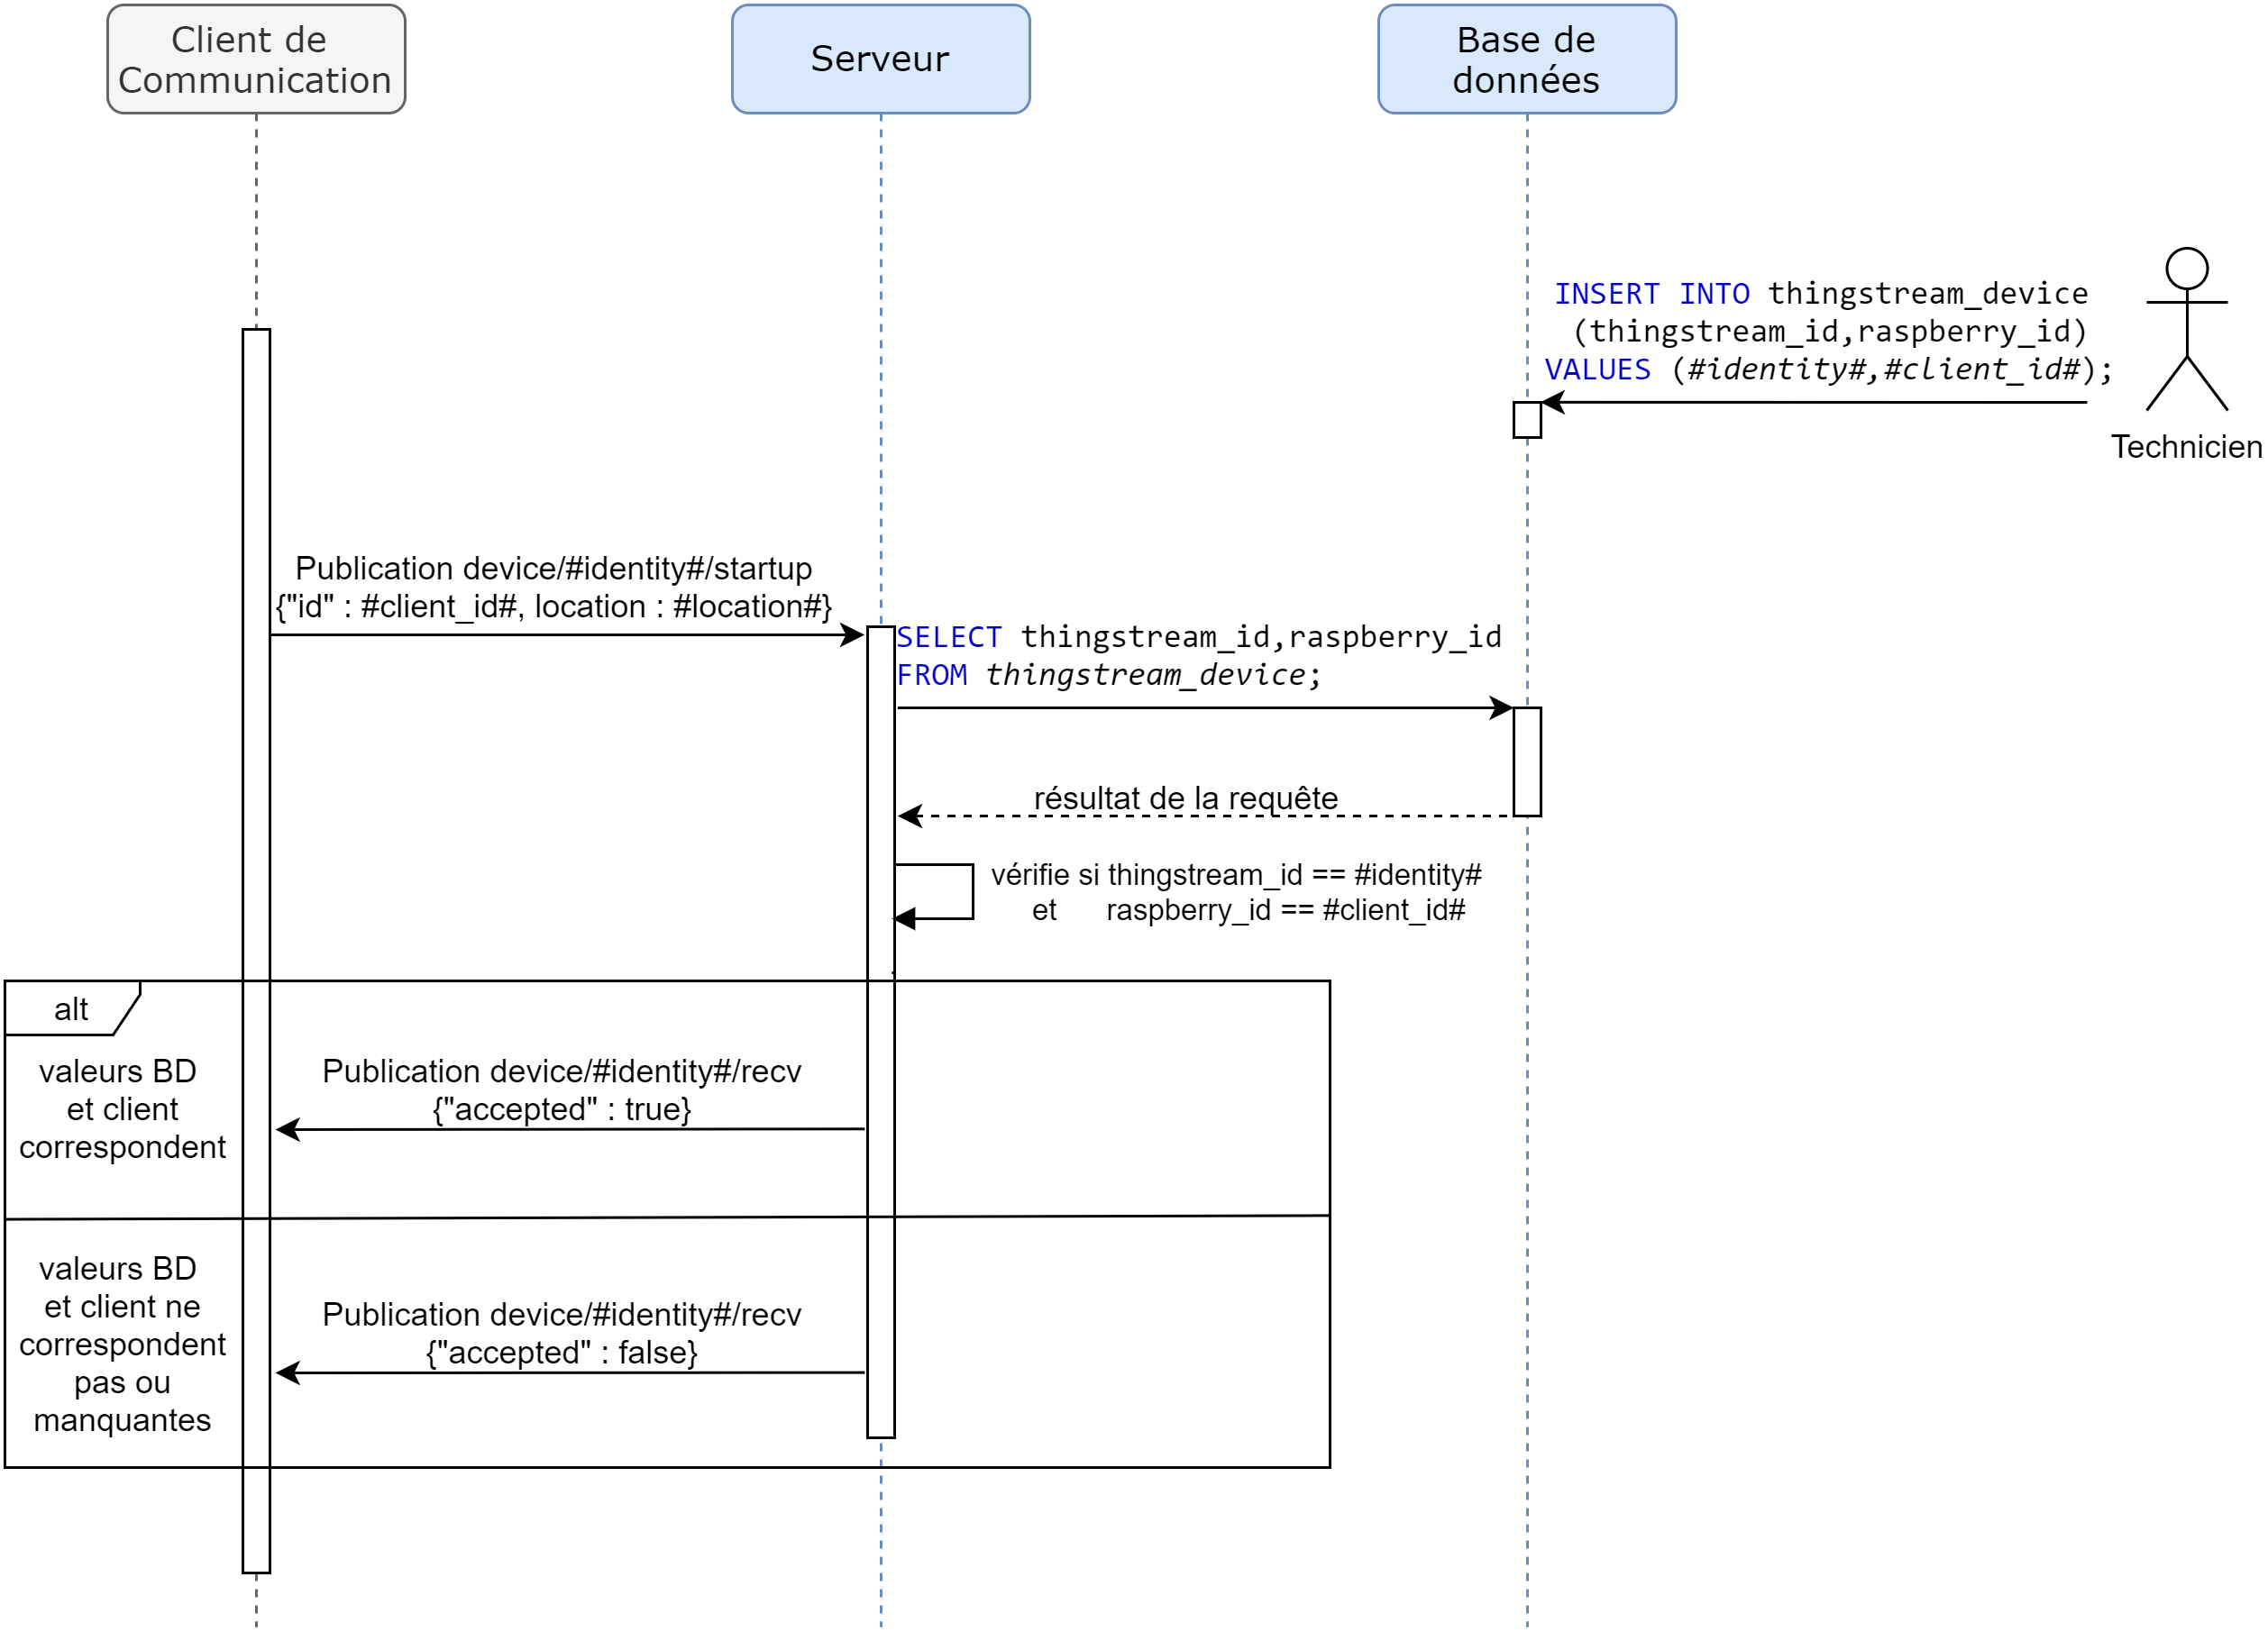
\includegraphics[width=\textwidth]{img/app/verify_identity.png}
  \caption{Processus de vérification de l'identité d'une application par le serveur. Ce diagramme complémente celui de la figure \ref{fig:seq111}}
  \label{fig:auth_app_server}
\end{figure}

\newpage

\subsubsection{Interface graphique}

\noindent
Le dernier point lié à l'application du serveur correspond à l'outil de visualisation de données. Il est primordial que les techniciens puissent vérifier l'état de l'infrastructure de CERHIS et trouver la source de la défaillance, s'il y en a une. En conséquence, un outil adapté aux données du projet est requis. Ils peuvent être classés sous trois grandes catégories : les bibliothèques logicielles, les dashboard, et les outils Business Intelligence (voir section \ref{sec:data_vis}).

~

\noindent
Les outils Business Intelligence ont été abandonnés en premier. Généralement, leur utilisation est associée avec un coût élevé et la quantité de données traitée actuellement ne requiert pas l'emploi d'un tel outil. En outre, le cahier des charges ne spécifie pas la nécessité de trouver une tendance dans les données.

~

\noindent
La décision se portait donc sur l'emploi d'un d'un outil \textit{dashboard} ou d'une bibliothèque logicielle. Cette dernière permet de créer une solution complètement customisée pour le projet, tirant le meilleur parti des données. En revanche, partir sur cette route demande une charge de travail importante. Il y a toute une logistique associée à cette approche comme le développement d'un site web, ou le choix de la meilleure manière pour afficher les données. En particulier, pour ce dernier point, il faut prendre en compte les 3 principes d'un bon outil de visualisation de données. (Fiables, Accessibles, et Élégantes).

~

\noindent
Ces mêmes principes doivent être suivis lors de l'emploi d'un outil \textit{dashboard}. Mais, le grand avantage est que ces outils aident l'utilisateur à accomplir cet objectif en offrant déjà certaines visualisations prédéfinies. De plus, ces affichages peuvent s'ajuster automatiquement aux données (par exemple les axes d'un graphique). Finalement, les \textit{dashboard} possèdent aussi un certain degré de customisation afin de laisser l'utilisateur adapter la visualisation à ses besoins. Tout cela est souvent proposé sous la forme d'un logiciel facile à installer et ne demandant pas de connaissances en programmation. \footnote{La manipulation des langages de requête (SQL) peut être nécessaire si la requête souhaitée ne peut être construite à l'aide de constructeurs de requêtes(\textit{query builders}).} Le problème majeur réside dans le fait que ces outils peuvent parfois ne pas offrir un certain affichage qui est recherché.

~

\noindent
Enfin, Grafana a été choisi comme solution de visualisation. Cet outil \textit{dashboard} s'est montré simple à manipuler lors de sa configuration pour la partie du client et l'utiliser pour le serveur permet d'avoir un ensemble de solutions plus homogène. De plus, il est compatible avec la base de données MySQL choisie antérieurement. À ce stade du prototype, créer une solution customisée n'est pas le choix le plus pertinent. L'application du serveur risque d'évoluer énormément durant les prochaines étapes si de nouvelles révisions sont apportées au client. Partir d'un \textit{dashboard} offre une immense flexibilité, car la visualisation peut être modifiée en une question de minutes, contrairement à l'utilisation d'une bibliothèque logicielle.

~

\noindent
À l'avenir, Grafana pourrait être remplacé si ce choix s'avère être un facteur limitant du projet, mais étant donné le grand nombre de plugins disponibles et qui ne fait qu'augmenter, cela pourrait ne jamais arriver.


\begin{figure}[ht!]
  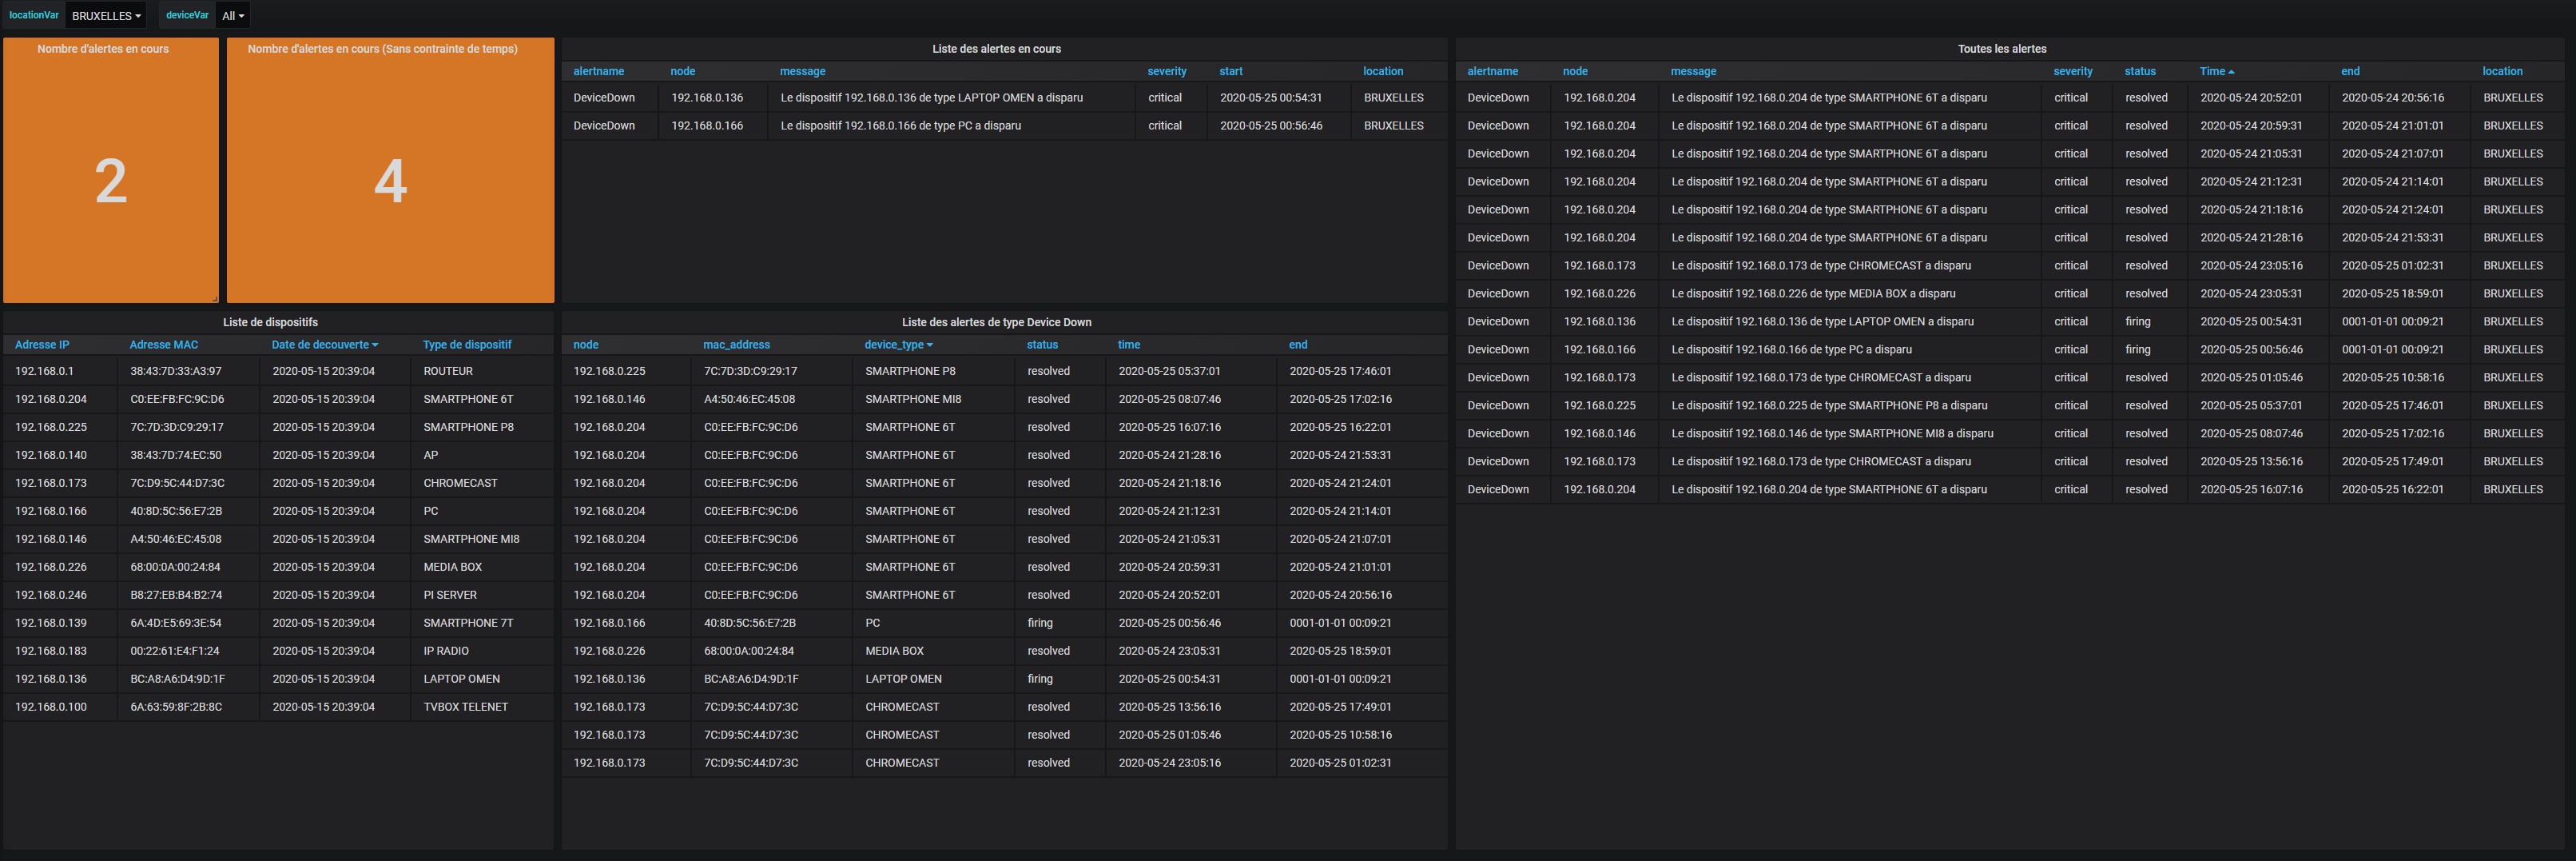
\includegraphics[width=\textwidth]{img/app/grafana_server.png}
  \caption{Interface de visualisation de données du serveur distant}
  \label{fig:graf_server}
\end{figure}

\subsection{Sécurité}

\noindent
Contrairement au client, le serveur a un accès à Internet. Le chiffrement des données devient beaucoup plus important afin de protéger les échanges d'informations. En particulier, les identifiants requis pour se connecter à Grafana ne doivent en aucun cas être transmis sur Internet sans utiliser des méthodes de cryptographie. De ce fait, le protocole TLS a été employé pour sécuriser la communication entre tous les composants du logiciel. La figure \ref{fig:ssl} montre le fonctionnement de ce protocole. Une fois qu'une connexion est établie entre \underline{deux parties} (\underline{client-serveur}), les \underline{deux instances} échangent des clés de chiffrement qui seront utilisées pour crypter les données. En outre, le \underline{serveur} envoie également un certificat qui permet de vérifier son identité auprès d'une tierce partie de confiance (l'instance qui a délivré le certificat).  Cette vérification évite que des attaques de l'homme du milieu (voir figure \ref{fig:middle}) puissent avoir lieu.


\begin{figure}[ht!]
  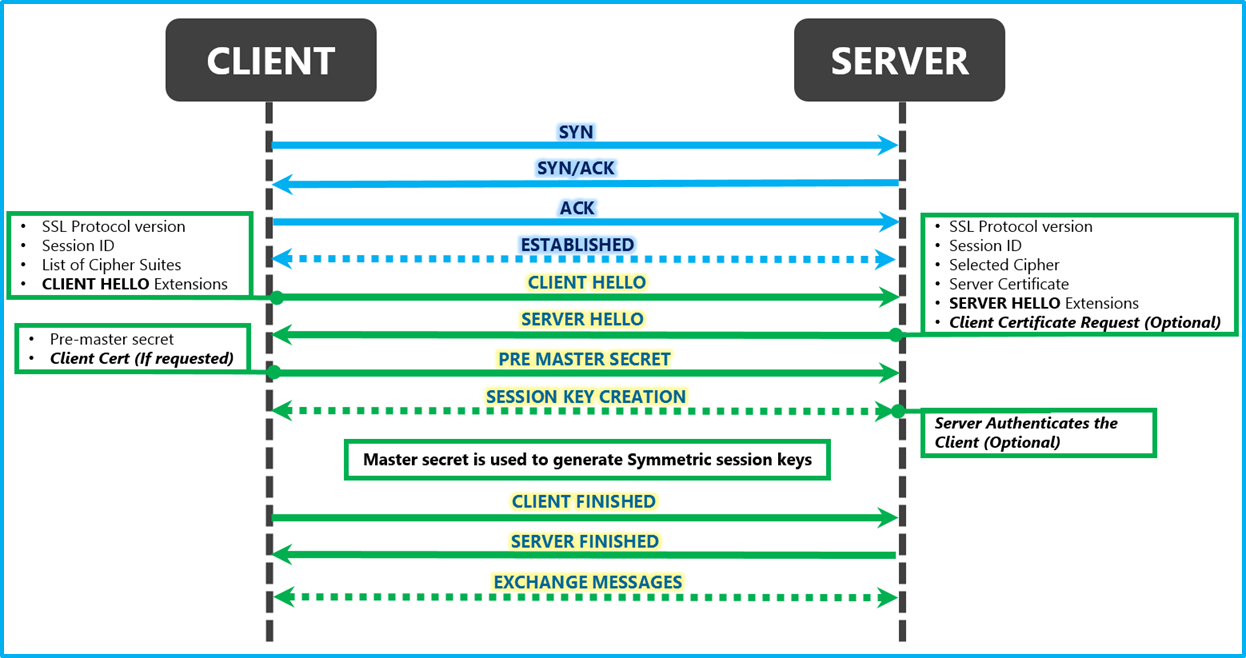
\includegraphics[width=\textwidth]{img/app/ssl.png}
  \caption{Digramme du déroulement du protocole TLS\cite{ssl_img}}
  \label{fig:ssl}
\end{figure}

\begin{figure}[ht!]
  \centering
  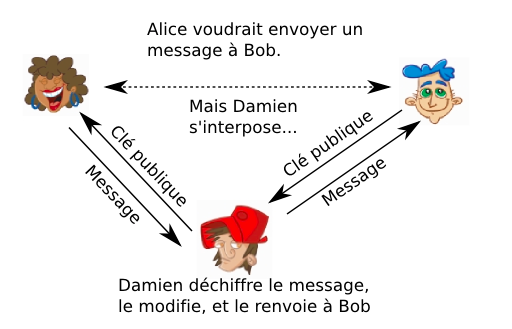
\includegraphics[width=0.7\textwidth]{img/app/man_in_the_middle.png}
  \caption{Exemple d'une attque de l'homme du milieu\cite{man_middle_img}}
  \label{fig:middle}
\end{figure}

\noindent
La figure \ref{fig:crypto} illustre où le protocole est déployé dans la solution implémentée dans ce mémoire. Veuillez noter que les certificats utilisés par la base de données et Grafana ont été autosignés. Ils ne protègent pas le \underline{client} contre des attaques de l'homme du milieu, mais leur utilisation est gratuite. Ils peuvent donc être exploités pendant la phase de développement pour éviter des coûts non nécessaires. Lors du déploiement de la solution complète, un certificat signé par une tierce partie de confiance peut être acquis pour remplacer les certificats autosignés


\begin{figure}[ht!]
  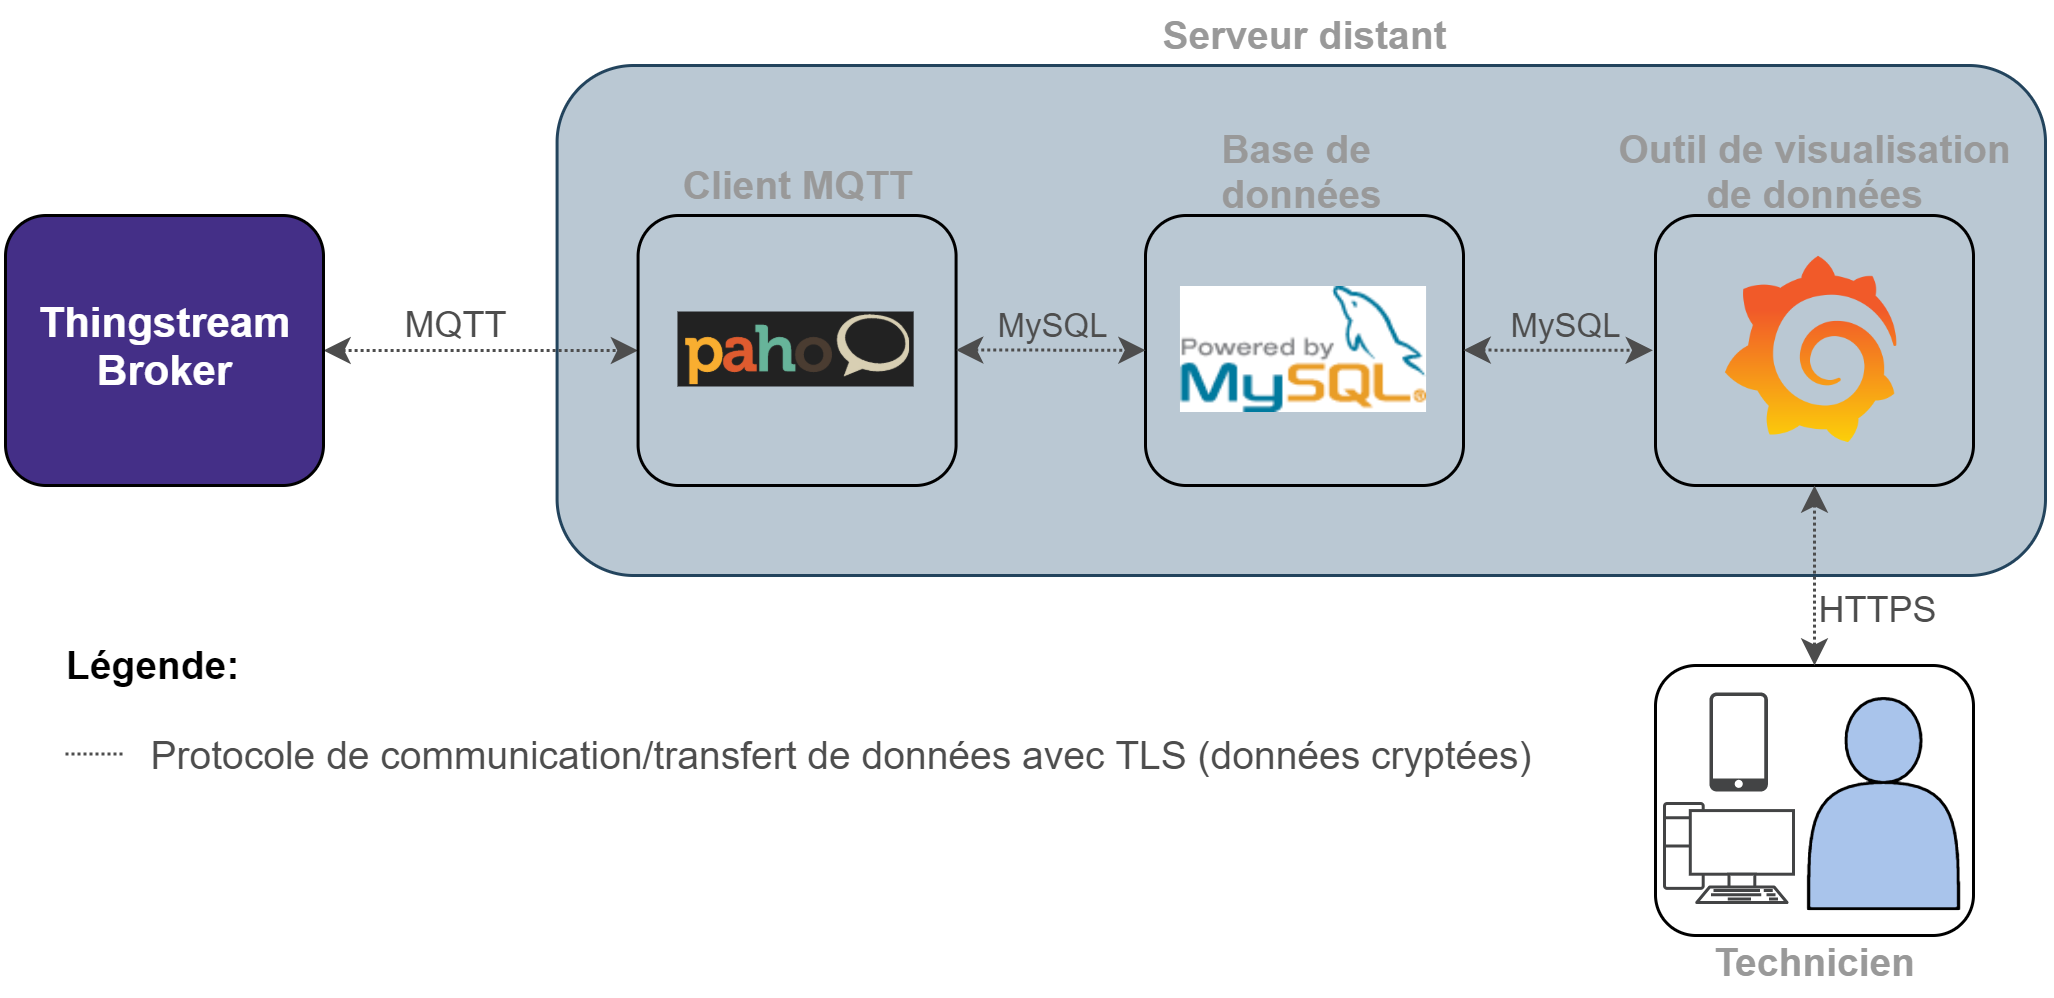
\includegraphics[width=\textwidth]{img/app/end_game.png}
  \caption{Architecture finale de l'application tournant sur le serveur distant}
  \label{fig:crypto}
\end{figure}
